\documentclass{jknotes}
\usepackage{../joshkirklin}

\setmathfont{Latin Modern Math}
\setmathfont{GFS NeoHellenic Math}[range=bfsfup/{greek,Greek}->it]
\setmathfont{GFS NeoHellenic Math}[range=sfup/{latin,Latin}->it]

\usetikzlibrary{shapes.misc, pgfplots.fillbetween}
\renewcommand{\u}{\symbf{u}}
\newcommand{\U}{\symbf{U}}
\newcommand{\Ra}{\text{Ra}}
\newcommand{\ReN}{\text{Re}}
\newcommand{\zint}{\int_{z_1}^{z_2}}
\newcommand{\veps}{\varepsilon}
\renewcommand{\y}{\symbf{y}}
\renewcommand{\L}{\mathcal{L}}
\renewcommand{\k}{\symbf{k}}
\renewcommand{\v}{\symbf{v}}

\tikzset{cross/.style={cross out, draw=black, minimum
size=2*(#1-\pgflinewidth), inner sep=0pt, outer sep=0pt}}
%default radius will be 1pt. 

\newcommand{\myol}[2][3]{{}\mkern#1mu\overline{\mkern-#1mu#2}}

\begin{document}

\institution{Cambridge Part III Maths}
\title{Hydrodynamic Stability}
\lecturer{Prof. Richard Kerswell}
\notetaker{Charles Powell}
\date{Lent 2021}

\maketitle
\suggestionsspiel
\tableofcontents

\section{Introduction}
We are typically interested in whether a given flow solution $\u(\x,t)$ is
`stable', certainly to small (infinitesimal) disturbances and perhaps to
larger perturbations too. We perturb $\u(\x)$ to $\u(\x) + \hat{\u}(\x,t)$ and
define the \emph{perturbation energy} as
\begin{equation}
	E(t) \equiv \int \frac{1}{2}\hat{\u}^2(\x,t) \, \diffd V
\end{equation}
A solution is said to be stable if
\begin{equation}
	\lim_{t \to \infty} \frac{E(t)}{E(0)} = 0
\end{equation}
for all perturbations $\hat{\u}$. Conversely, if there exists $\hat{\u}$ such
that $E(t) \not\rightarrow 0$ then $\u$ is unstable. The nature of $E(0)$
determines the type of perturbation:
\begin{itemize}
	\item If $E(0) \to 0$ we have an infinitesimal disturbance
	\item If $E(0) < \delta$ then we probe finite amplitude disturbances
	\item If $E(0) \to \infty$ this probes the \emph{global} stability
\end{itemize}

In the first 9 lectures we focus on the first situation, which is linear
stability analysis. Consider the Navier-Stokes equations
\begin{align}
	\frac{\partial \u}{\partial t} + \u \cdot \nabla \u + \nabla p =
	\frac{1}{\text{Re}} \nabla^2 \u
\end{align}

If $\symbf{U}(\x)$ is a steady (basic) solution then
\begin{equation}
	\symbf{U}\cdot\nabla\symbf{U} + \nabla P = \frac{1}{\text{Re}} \nabla^2
	\symbf{U}
\end{equation}
Let $\u = \symbf{U}(\x) + \hat{\u}(\x,t), p = P + \hat{p}$. Then
\begin{equation}
	\frac{\partial \hat{\u}}{\partial t} + \u \cdot \nabla \symbf{U} +
	\symbf{U} \cdot \nabla \hat{\u} + \cancel{\hat{\u}\cdot\nabla\hat{\u}} +
	\nabla \hat{p} = \frac{1}{\text{Re}} \nabla^2 \hat{\u}
\end{equation}
The term $\hat{u}\cdot\nabla \symbf{U}$ is stabilising whilst the term
$\nabla^2 \hat{u} / \text{Re}$ is destabilising. Therefore, we expect stability
as $\text{Re} \to 0$ the stabilising term dominates, and instability as
$\text{Re} \to \infty$ when the destablising term dominates. Thus there exists
some value $\text{Re}_{\text{crit}}$ at which instability arises. We will ask
what this value is, and what is the form of the initial
instability/mode/pattern?

\section{Kelvin-Helmholtz instability}
See Drazin (2002), section 3.3, pages 47--50. Here we take a different approach
and derive Rayleigh's equation (example 8.3, page 151 of Drazin). 

\begin{center}
	\begin{tikzpicture}
		\draw[thick,->] (-3, 0) -- (3, 0) node[right] {$x$};
		\draw[dashed,->] (0, -1.5) -- (0, 1.5) node[above] {$z$};
		\draw[blue,dashed] (1.5, 0) -- (1.5, 1.4);
		\draw (1.5, 0) node[below] {$U$};
		\draw (-1.5, 0) node[above] {$-U$};
		\draw[blue,dashed] (-1.5, 0) -- (-1.5, -1.4);

		\draw[blue,->] (0, 0.4) -- (1.5, 0.4);
		\draw[blue,->] (0, 0.8) -- (1.5, 0.8);
		\draw[blue,->] (0, 1.2) -- (1.5, 1.2);
		\draw[blue,->] (0, -0.4) -- (-1.5, -0.4);
		\draw[blue,->] (0, -0.8) -- (-1.5, -0.8);
		\draw[blue,->] (0, -1.2) -- (-1.5, -1.2);
	\end{tikzpicture}
\end{center}

Consider a flow $\u = U(z)\hat{\x}$ where
\begin{equation}
	U(z) = \begin{cases} U & z > 0 \\ -U & z < 0 \end{cases}
\end{equation}
The linearised, \emph{inviscid} equation for perturbation $\hat{\u}$ is
\begin{align}
	\frac{\partial \hat{\u}}{\partial t} + \hat{w}U'\hat{\x} + U
	\frac{\partial \hat{\u}}{\partial x} + \nabla \hat{p} &= 0 \\
	\nabla \cdot \hat{\u} &= 0 
\end{align}
The boundary conditions are $\hat{\u} \to 0$ as $z \to \pm \infty$, i.e. no
energy is radiated in from infinity. We will work in 2D with velocity
components $(\hat{u},\hat{w}) = (\psi_z, -\psi_x)$ and let $\psi(x,z,t) =
\phi(z) e^{i\alpha(x-ct)}$ where $c$ is a complex eigenvalue, currently
unknown. Formally, this is equivalent to taking a Fourier transform. We have
\begin{equation}
	i\alpha (U-c) \begin{pmatrix} \phi' \\ -i\alpha \phi \end{pmatrix} +
	\begin{pmatrix} -i\alpha U' \phi \\ 0 \end{pmatrix} + \begin{pmatrix} i
\alpha p \\ \frac{\partial p}{\partial z} \end{pmatrix} = 0
\end{equation}
We can eliminate $p$ via $\partial_z (\text{top}) - i\alpha(\text{bottom})$ to
get
\begin{equation}
	(U-c)(\phi''-\alpha^2 \phi) - U'' \phi = 0
\end{equation}
with boundary conditions $\phi \to 0$ as $z \to \pm \infty$. This is
\emph{Rayleigh's equation}. Note that $c$ is the crucial eigenvalue. We wish to
know when $c_i = \Im(c) > 0$ as a function of $U(z)$, as $c_i$ is the growth
rate:
\begin{equation}
	\hat{u} \propto e^{i\alpha(x-ct)} = e^{i\alpha(c-c_r t - i c_i t)} =
		e^{i\alpha(x-c_r t) + \alpha c_i t}
\end{equation}
Note the following:
\begin{itemize}
	\item There is a symmetry $\alpha \mapsto -\alpha$, so without loss of
		generality we consider $\alpha > 0$.
	\item The complex conjugate is also a solution with $c \mapsto c^*$. Hence
		an unstable mode has a damped partner, so we have stability only if
		all modes are `neutral' i.e. $c_i = 0$. 
	\item There is a possible singularity at $y$ where $U(y) = c$, called the
		\emph{critical layer}. If $c$ is real, see later.
\end{itemize}

We now solve Rayleigh's equation with $U(z)$ defined as before. We solve above
and below $z=0$ and piece the solutions together. Since $U'' = 0$, we have
\begin{equation}
	\phi'' = \alpha^2 \phi
\end{equation}
which admits a solution satisfying the boundary conditions:
\begin{equation}
	\phi = \begin{cases} A^{-\alpha z} & z > 0 \\ B e^{\alpha z} & z < 0 
	\end{cases}
\end{equation}

The matching conditions at $z=0$ are
\begin{enumerate}
	\item Pressure $\hat{p}$ continuous at $z=0$, with $\hat{p}$ given by:
		\begin{equation}
			\hat{p} = U' \phi - (U-c) \phi'
		\end{equation}
	\item Kinematic condition at the surface:
		\begin{equation}
			\frac{\diffD}{\diffD t} \left( z - \zeta(x,t)\right) = 0
		\end{equation}
		where $z=\zeta(x,t)$ is the position of the surface.
		After linearising, we have
		\begin{equation}
			 w - \frac{\partial \zeta}{\partial t} - U\frac{\partial
			 \zeta}{\partial x} = 0
		\end{equation}
	 	Inserting the form of $w$ and $U$ we require that
	 	\begin{equation}
		 	\zeta = - \frac{\phi}{U-c}
	 	\end{equation}
	 	is continuous across $z=0$.
\end{enumerate}
Requiring $p$ continuous gives
\begin{equation}
	-(U-c)A(-\alpha) = - (-U-c)B(\alpha)
\end{equation}
Requiring $\zeta$ continuous gives
\begin{equation}
	\frac{A}{U-c} = \frac{B}{-U-c}
\end{equation}
Hence we have
\begin{equation}
	(U-c)^2 = -(U+c)^2
\end{equation}
i.e. $c = \pm i U$ so the growth rate is $\alpha U$. Thus the flow is unstable
to waves of all wavelengths. The instability may be remedied 
\begin{itemize}
	\item by adding a density stratification, which stabilises long
		wavelengths (small $\alpha$)
	\item by adding surface tension, which stabilises short wavelengths (large
		$\alpha$), e.g. Drazin page 50 equation 3.21.
\end{itemize}

\section{Thermal instabilities: Rayleigh-Bernard convection}
Consider two parallel plates separated by distance $L$ with fluid subject to
gravity and temperatue difference $\Delta T$ between the plates. The lower
plate is heated to $T_0 + \Delta T$ whilst the upper plate is fixed at
temperature $T_0$. 
\begin{center}
	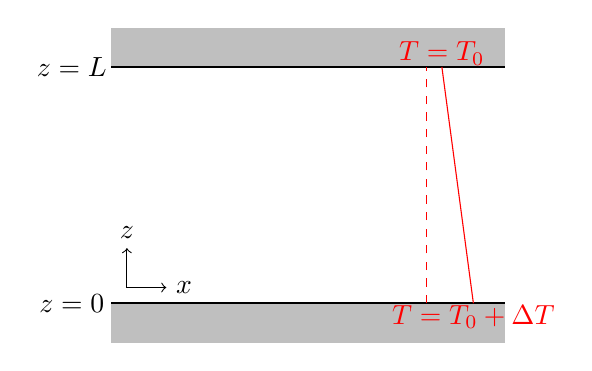
\begin{tikzpicture}
		\draw[draw=none,fill=gray!50] (0,0) rectangle (5,-0.5);
		\draw[thick] (0,0) -- (5, 0);
		\draw[draw=none,fill=gray!50] (0,3) rectangle (5,3.5);
		\draw[thick] (0,3) -- (5, 3);

		\draw[->] (0.2, 0.2) -- (0.7, 0.2) node[right] {$x$};
		\draw[->] (0.2, 0.2) -- (0.2, 0.7) node[above] {$z$};
		\draw (-0.5, 0) node {$z=0$};
		\draw (-0.5, 3) node {$z=L$};
		\draw[red,dashed] (4, 0) -- (4, 3);
		\draw[red] (4.2, 3) -- (4.6, 0);
		\draw[red] (4.2, 2.9) node[above] {$T=T_0$};
		\draw[red] (4.6, 0.1) node[below] {$T=T_0+\Delta T$};
	\end{tikzpicture}
\end{center}

The basic state consists of no motion, with heat transfer by conduction only.
\paragraph{Governing equations.}
The governing equations are those of momentum, mass, and (thermal) energy
conservation.
\begin{align}
	\rho \frac{\diffD \u}{\diffD t} + \nabla p &= \mu \nabla^2 \u + \rho g
	\hat{\symbf{z}} \\
	\frac{\partial T}{\partial t} + \u \cdot \nabla T &= \kappa \nabla^2 T \\
	\frac{\diffD \rho}{\diffD t} + \rho \nabla \cdot \u &= 0
\end{align}
To close the set of equations we need a relationship between $\rho$ and $T$.
Most cases of interest have $\Delta T$ and $\Delta \rho$ small, i.e. $\Delta
\rho \ll \rho_0, \Delta T \ll T_0$. Two consequences of this assumption are:
\begin{enumerate}
	\item We can Taylor expand $\rho = \rho(T)$:
		\begin{equation}
			\rho \approx \rho(T_0) \left[ 1 - \alpha(T-T_0)\right]
		\end{equation}
		where $\alpha > 0$ is the coefficient of thermal expansion, such that
		$T$ increases when $\rho$ decreases. We write $\rho_0 = \rho(T_0)$.
	\item We can adopt a Boussinesq approximation: acknowledge density changes
		only in the buoyancy term $\rho g \hat{\symbf{z}}$. Importantly, we
		can assume the fluid is incompressible.
\end{enumerate}

Define $\theta = T - T_0$. The governing equations are now
\begin{align}
	\rho_0 \frac{\diffD \u}{\diffD t} + \nabla p &= \mu \nabla^2 \u +
	\rho_0(1-\alpha \theta)g \hat{\symbf{z}} \\
	\frac{\partial \theta}{\partial t} + \u \cdot \nabla \theta &= \kappa
	\nabla^2 \theta \\
	\nabla \cdot \u &= 0
\end{align}

The basic state is $u = 0, \theta = \Delta T (1-z/L)$ and
\begin{equation}
	\frac{\diffd p}{\diffd z} = -\rho_0 (1-\alpha \Delta T(1-z/L))g
\end{equation}

We now non-dimensionalise using scalings $t \sim L^2/\kappa, u \sim \kappa/L,
\theta \sim \Delta T$, e.g. $\theta = \Delta T \theta^*$ where $\theta^*$ is
the non-dimensionalised variable. We normalise the $\frac{\diffD \u^*}{\diffD
t^*}$ term, to get:
\begin{align}
	\frac{\diffD \u^*}{\diffD t^*} + \nabla^* p^* &= \frac{\mu}{\rho_0 \kappa}
	\nabla^{*2} \u^* + \frac{\alpha g \Delta T L^3}{\kappa^2} \theta^* \hat{\symbf{z}} \\
	\frac{\partial \theta^*}{\partial t^*} + \u^* \cdot \nabla^* \theta^* &=
	\nabla^{*2} \theta^* \\
\end{align}
Define the \emph{Prandtl number} 
\begin{equation}
	\sigma \equiv \frac{\nu}{\kappa} = \frac{\mu}{\rho_0 \kappa}
\end{equation}
which is the ratio of viscous/momentum diffusion to thermal diffusion. Typical values
are $0.72$ in air, $7$ in water, $10^5$ in magma. We also define the
\emph{Rayleigh number}
\begin{equation}
	\text{Ra} \equiv \frac{\alpha \Delta T g L^3}{\kappa \nu}
\end{equation}
which is the ratio of destabilising buoyancy to stabilising diffusion.
Dropping the $^*$ notation, we have
\begin{align}
	\frac{\partial \u}{\partial t} + \u \cdot \nabla \u + \nabla p &= \sigma
	\nabla^2 \u + \sigma \text{Ra} \theta \hat{\symbf{z}} \\
	\frac{\partial \theta}{\partial t} + \u \cdot \nabla \theta &= \nabla^2
	\theta \\
	\nabla \cdot \u &= 0
\end{align}

\paragraph{Boundary conditions.}
There are three combinations of boundary condition available in this problem,
with the choice fixed wall (no slip) or stress free (free slip).
\begin{center}
	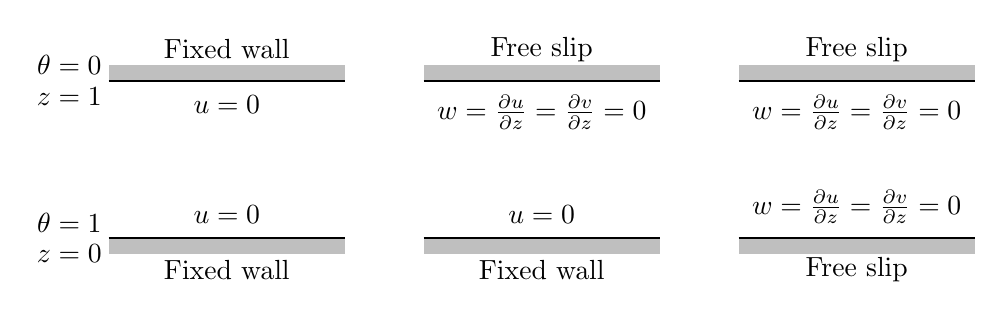
\begin{tikzpicture}
		\draw (-0.5, 0.2) node {$\theta = 1$};
		\draw (-0.5, -0.2) node {$z = 0$};
		\draw (-0.5, 2.2) node {$\theta = 0$};
		\draw (-0.5, 1.8) node {$z = 1$};

		\draw[fill=gray!50,draw=none] (0,0) rectangle (3,-0.2);
		\draw[fill=gray!50,draw=none] (0,2) rectangle (3,2.2);
		\draw[thick] (0,0) -- (3, 0);
		\draw[thick] (0,2) -- (3, 2);

		\draw (1.5, 0.3) node {$\u = 0$};
		\draw (1.5, 1.7) node {$\u = 0$};

		\draw (1.5, -0.4) node {Fixed wall};
		\draw (1.5, 2.4) node {Fixed wall};

		\begin{scope}[shift={(4, 0)}]
			\draw[fill=gray!50,draw=none] (0,0) rectangle (3,-0.2);
			\draw[fill=gray!50,draw=none] (0,2) rectangle (3,2.2);
			\draw[thick] (0,0) -- (3, 0);
			\draw[thick] (0,2) -- (3, 2);

			\draw (1.5, 0.3) node {$\u = 0$};
			\draw (1.5, 1.6) node {$w = \frac{\partial u}{\partial z} =
			\frac{\partial v}{\partial z} = 0$};

			\draw (1.5, -0.4) node {Fixed wall};
			\draw (1.5, 2.4) node {Free slip};
		\end{scope}
		\begin{scope}[shift={(8, 0)}]
			\draw[fill=gray!50,draw=none] (0,0) rectangle (3,-0.2);
			\draw[fill=gray!50,draw=none] (0,2) rectangle (3,2.2);
			\draw[thick] (0,0) -- (3, 0);
			\draw[thick] (0,2) -- (3, 2);

			\draw (1.5, 1.6) node {$w = \frac{\partial u}{\partial z} =
			\frac{\partial v}{\partial z} = 0$};
			\draw (1.5, 0.4) node {$w = \frac{\partial u}{\partial z} =
			\frac{\partial v}{\partial z} = 0$};

			\draw (1.5, -0.4) node {Free slip};
			\draw (1.5, 2.4) node {Free slip};
		\end{scope}
	\end{tikzpicture}
\end{center}

The double fixed wall case is easiest to replicate in a lab, whilst the double
free slip case is the easiest analytically, which we shall use.

\paragraph{Basic state.}
In the basic state we have conductive profile $\u_0 = 0, \theta_0 = 1-z$ and
from integration $p_0 = \sigma \text{Ra}( z - \frac{1}{2}z^2)$. We generate
linearised equations for perturbations $\theta = \theta_0 + \theta', \u = \u_0
+ \u', p = p_0 + p'$. As usual with linear stability analysis, we assume
$(\theta', \u', p')$ are small.

\begin{align}
	\frac{\partial \u'}{\partial t} + \cancel{\u' \cdot \nabla \u'} + \nabla
	p' &= \sigma \nabla^2 \u' + \sigma \text{Ra} \theta' \hat{\symbf{z}} \\
	\frac{\partial \theta'}{\partial t} - w' + \cancel{\u' \cdot \nabla
	\theta'} &= \nabla^2 \theta' \\
	\nabla  \cdot \u' &= 0 
\end{align}

Dropping the $'$ notation for clarity we have perturbation equations
\begin{align}
	\left( \frac{\partial}{\partial t} - \sigma \nabla^2\right)\u + \nabla p =
	\sigma \text{Ra} \theta \hat{\symbf{z}} \label{eq:therm:1}\\
	\nabla \cdot \u &= 0 \label{eq:therm:2}\\
	\left( \frac{\partial}{\partial t} - \nabla^2\right)\theta &= w
	\label{eq:therm:3}
\end{align}

The perturbation boundary conditions also follow by inserting variables into
the total boundary conditions, e.g. $\theta = \theta_0 + \theta' = 1$ at $z=0$
combined with $\theta_0 = 1$ at $z=0$ gives $\theta' = 0$. Similarly, $\theta'
= 0$ at $z=1$ and in fact all boundary conditions are homogeneous. To proceed
further, we need to reduce the equations \eqref{eq:therm:1},\eqref{eq:therm:2}
and \eqref{eq:therm:3} into a single equation.

From $\nabla \times \eqref{eq:therm:1}$ we have
\begin{equation}
	\left( \frac{\partial}{\partial t} - \sigma \nabla^2\right)\symbf{\omega}  =
	\sigma \text{Ra} \nabla \times \theta \hat{\symbf{z}}
\end{equation}
Taking the curl again and using $\nabla \times \symbf{\omega} = \nabla \times
(\nabla \times \u) = \nabla (\nabla \cdot \u) - \nabla^2 \u$ we have
\begin{equation}
	\left(\frac{\partial}{\partial t} - \sigma \nabla^2 \right) (-\nabla^2 \u)
	= \sigma \text{Ra} \nabla \times (\nabla \times \theta \hat{\symbf{z}}) =
	\sigma \text{Ra} \left( \nabla \frac{\partial \theta}{\partial z} -
	\hat{\symbf{z}} \nabla^2 \theta \right)
\end{equation}
The $z$ component is
\begin{equation}
	\left(\frac{\partial}{\partial t} - \sigma \nabla^2 \right) (-\nabla^2 w)
	= \sigma \text{Ra} \nabla_H^2 \theta
	\label{eq:therm:4}
\end{equation}
where $\nabla_H^2 = \partial_x^2 + \partial_y^2$. Now \eqref{eq:therm:3} can
be used to eliminate $\theta$ by applying the operator $(\partial_t -
\nabla^2)$:
\begin{equation}
	\left(\frac{\partial}{\partial t} - \sigma \nabla^2
	\right)\left(\frac{\partial}{\partial t} - \nabla^2\right)\nabla^2 w =
	\sigma \text{Ra} \nabla_H^2 w
	\label{eq:therm:5}
\end{equation}
This is a 6\textsuperscript{th} order PDE for $w$, hence we need three
boundary conditions at each wall $z=0,1$. We use stress-free (i.e. free slip)
at both walls to simplify analysis. Thus we have
\begin{equation}
	\frac{\partial u}{\partial z} = \frac{\partial v}{\partial z} = w = 0
	\hspace{2em} \text{at} \,\,\, z=0,1
\end{equation}
The second set of conditions comes from incompressibility. Taking $\partial_z
(\nabla \cdot \u)$ we have
\begin{equation}
	\frac{\partial}{\partial x} \left(\frac{\partial u}{\partial z}\right) +
	\frac{\partial}{\partial y} \left(\frac{\partial v}{\partial z}\right) +
	\frac{\partial^2 w}{\partial z^2} = 0 \implies w_{zz} = 0 
\end{equation}
The third and final set of conditions comes from requiring $\theta = 0$ at
$z=0,1$. From \eqref{eq:therm:4}, $\nabla_H^2 \theta = 0$ implies
\begin{equation}
	\left(\frac{\partial}{\partial t} - \sigma \nabla^2\right) \nabla^2 w = 0
\end{equation}
We now have 6 boundary conditions to supplement the PDE.

\paragraph{Normal mode solution.}
Seek a solution $w(x,y,z,t) = W(z) e^{ik_1x+ik_2y+\lambda t}$ where $k_1, k_2$
are wavenumbers and $\lambda \in \mathbb{C}$ is the growth rate. Write $D =
\diffd/\diffd z$ and $k = \sqrt{k_1^2+k_2^2}$ since the problem is
rotationally symmetric in the $(x,y)$ plane. Substituting into
\eqref{eq:therm:5} we have
\begin{equation}
	(\lambda - \left[ D^2 - k^2 \right])(\lambda - \sigma \left[ D^2 -
	k^2\right])(D^2-k^2)W = - \sigma \text{Ra}k^2 W
\end{equation}
with boundary conditions at $z=0,1$:
\begin{align}
	W(0) = W(1) &= 0 \\
	D^2 W(0) = D^2 W(1) &= 0 \\
	\left[ \lambda - \sigma (D^2 - k^2)\right]\left[D^2 - k^2\right] W = 0
	\implies D^4 W(0) = D^4 W(1) &= 0 
\end{align}

The objective is to find 
\begin{equation}
	\max_k \Re\{ \lambda(k;\Ra,\sigma)\}
\end{equation}
The onset of linear instability (for a given $\sigma$) at $\Ra =
\Ra_{\text{crit}}$ is defined by
\begin{equation}
	\max_k \Re\{\lambda(k; \Ra_{\text{crit}},\sigma)\} = 0
\end{equation}
In general, $\lambda \in \mathbb{C}$, but for this problem it can be proven
that at marginality $\Im(\lambda) = 0$ as well as $\Re(\lambda) = 0$; a
condition called the \emph{principle of exchange of stabilities}. Hence
setting $\lambda = 0$ in the above, we get
\begin{equation}
	(D^2 - k^2)^3 W = - \Ra \,k^2 W
	\label{eq:therm:6}
\end{equation}
Note that $\sigma$ drops out of the problem! It's easy to see $W(z) = \sin
(n\pi z)$ solves \eqref{eq:therm:6} and satisfies the free-slip BCs. Hence
\begin{equation}
	(n^2 \pi^2 + k^2)^3 = \Ra \,k^2
\end{equation}
Criticality is then given by
\begin{equation}
	\Ra_{\text{crit}} = \min_{n,k} \frac{(n^2 \pi^2 + k^2)^3}{k^2}
\end{equation}
We find the minimum in the usual way:
\begin{align}
	\frac{\partial \Ra}{\partial k} &= \frac{3(2k)(n^2\pi^2 + k^2)^2 k^2 -
	2k(n^2\pi^2 + k^2)^3}{k^4} \\
									&= \frac{2k(n^2\pi^2
									+k^2)^2(3k^2-(n^2\pi^2+k^2))}{k^4} = 0\\
		\implies 2k^2 &= n^2 \pi^2 \\
		\implies k &= \frac{n\pi}{\sqrt{2}}
\end{align}
Given $k = n\pi/\sqrt{2}$ the Rayleigh number is
\begin{equation}
	\Ra(k = \frac{n\pi}{\sqrt{2}}) = \frac{(n^2\pi^2 +
	\frac{1}{2}n^2\pi^2)^3}{n^2 \pi^2/2} = \frac{27}{4}n^4 \pi^4
\end{equation}
Clearly the critical Rayleigh number is given by $n=1$, hence
\begin{align}
	\Ra_{\text{crit}} &= \frac{27}{4}\pi^4 \sim 658 \\
	k_{\text{crit}} &= \frac{\pi}{\sqrt{2}} \sim 2.22
\end{align}

\begin{center}
	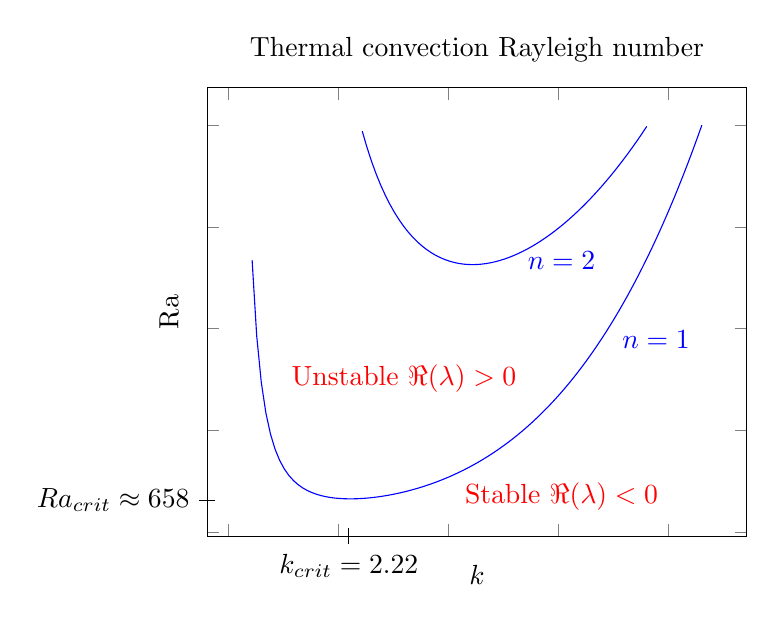
\begin{tikzpicture}
		\begin{axis}[title={Thermal convection Rayleigh
			number},ylabel={Ra},xlabel={$k$},yticklabels={,,},xticklabels={,,},
			samples=100,domain=0:10, restrict y to domain=0:8]
		%\draw[thick,->] (-0.1,0) -- (10, 0) node[right] {$k$};
		%\draw[thick,->] (0, -0.1) -- (0, 8) node[above] {Ra};
			\addplot[blue] plot[domain=0.353:8.611,samples=100] ({\x},{(pi^2 +
			\x^2)^3/(1000*\x^2)});
			\addplot[blue] plot[domain=0.353:8.611,samples=100] ({\x},{(4*pi^2 +
			\x^2)^3/(2000*\x^2)});
		\end{axis}
		\draw (0.1, 0.458) -- (-0.1, 0.458) node[left]
		{$\Ra_{\text{crit}} \approx 658$};
		\draw (1.8, 0.1) -- (1.8, -0.1) node[below] {$k_{\text{crit}} =
		2.22$};
		\draw[blue] (5.7, 2.5) node {$n=1$};
		\draw[blue] (4.5, 3.5) node {$n=2$};
		\draw[red] (4.5, 0.5) node {Stable $\Re(\lambda) < 0$};
		\draw[red] (2.5, 2) node {Unstable $\Re(\lambda) > 0$};
	\end{tikzpicture}
\end{center}

Results for other boundary conditions are:
\begin{itemize}
	\item Free--rigid boundary: $\Ra_{\text{crit}} \sim 1101, k_c = 2.68$
	\item Rigid--rigid boundary: $\Ra_{\text{crit}} \sim 1708, k_c = 3.117$
\end{itemize}

Notice that at criticality only the size of $k$ is specified, \emph{not} its
direction. Hence there are an infinite number of possibilities $\symbf{k} =
(k\cos\phi,k\sin\phi)$. Various different patterns which tesselate are as
follows.

\begin{enumerate}
	\item \textbf{2D rolls.} Orientate $x$-axis along $k$ such that $k_2 = 0$.
		We have velocity components ($w$ specified in problem, $u$ follows
		from incompressibility)
		\begin{align}
			w &= W(z) \sin kx \\
			v &= 0\\ 
			u &= \frac{\pi \cos \pi z \cos k x}{k}
		\end{align}

		\begin{center}
			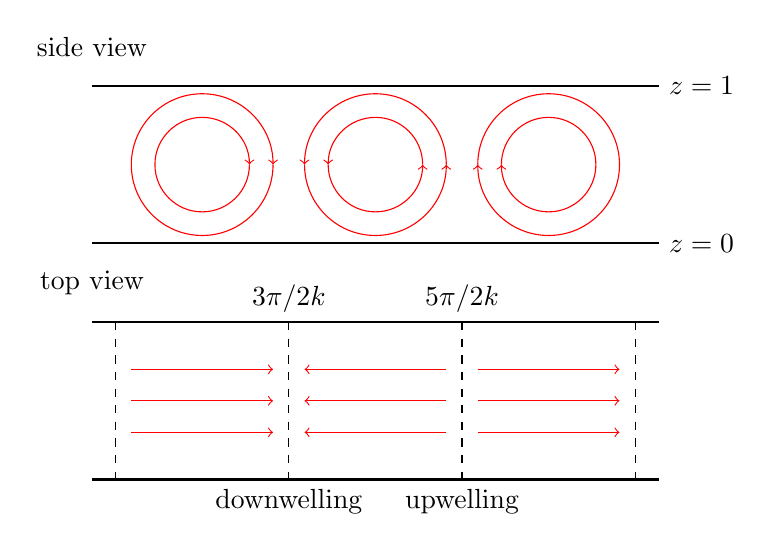
\begin{tikzpicture}
				\draw (0, 2.5) node {side view};
				\draw[thick] (0,0) -- (7.2, 0) node[right] {$z=0$};
				\draw[thick] (0,2) -- (7.2, 2) node[right] {$z=1$};
				\draw[red,<-] (2.3, 1) arc(0:360:0.9);
				\draw[red,<-] (2.0, 1) arc(0:360:0.6);
				\draw[red,->] (2.7, 1) arc(-180:0:0.9);
				\draw[red,->] (3.0, 1) arc(-180:0:0.6);
				\draw[red,->] (4.5, 1) arc(0:180:0.9);
				\draw[red,->] (4.2, 1) arc(0:180:0.6);
				\draw[red,<-] (4.9, 1) arc(-180:180:0.9);
				\draw[red,<-] (5.2, 1) arc(-180:180:0.6);
			\begin{scope}[shift={(0,-3)}]
				\draw (0, 2.5) node {top view};
				\draw[thick] (0,0) -- (7.2, 0);
				\draw[thick] (0,2) -- (7.2, 2);
				\draw[dashed] (2.5, 2) -- (2.5, 0) node[below] {downwelling};
				\draw[dashed] (4.7, 2) -- (4.7, 0) node[below] {upwelling};
				\draw[dashed] (6.9, 2) -- (6.9, 0);
				\draw[dashed] (0.3, 2) -- (0.3, 0);
				\draw (2.5, 2) node[above] {$3\pi/2k$};
				\draw (4.7, 2) node[above] {$5\pi/2k$};
				
				\draw[red,->] (0.5, 1.4) -- (2.3, 1.4);
				\draw[red,->] (0.5, 1) -- (2.3, 1);
				\draw[red,->] (0.5, 0.6) -- (2.3, 0.6);

				\draw[red,->] (4.5, 1.4) -- (2.7, 1.4);
				\draw[red,->] (4.5, 1) -- (2.7, 1);
				\draw[red,->] (4.5, 0.6) -- (2.7, 0.6);

				\draw[red,->] (4.9, 1.4) -- (6.7, 1.4);
				\draw[red,->] (4.9, 1) -- (6.7, 1);
				\draw[red,->] (4.9, 0.6) -- (6.7, 0.6);
			\end{scope}
			\end{tikzpicture}
		\end{center}
	\item \textbf{Rectangles.} Velocity components are
		\begin{align}
			w &= W(z) \cos k_1 x \cos k_2 y \\
			v &= -\frac{k_2}{k^2} W' \cos k_1 x \sin k_2 y \\
			u &= -\frac{k_1}{k^2} W' \sin k_1 x \cos k_2 y
		\end{align}
		\begin{center}
			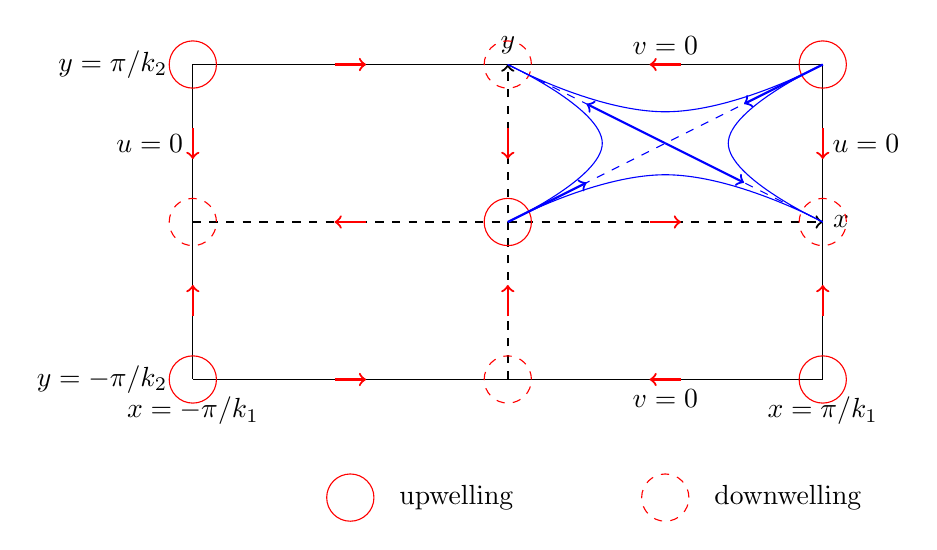
\begin{tikzpicture}
				\draw (0,0) -- (8,0) -- (8, 4) -- (0, 4) -- (0,0);
				\draw[dashed,thick,->] (4, 0) -- (4,4) node[above] {$y$};
				\draw[dashed,thick,->] (0, 2) -- (8,2) node[right] {$x$};

				\draw[blue,dashed] (4,2) -- (8, 4);
				\draw[blue,dashed] (4, 4) -- (8, 2);

				\draw[red,dashed] (0, 2) circle (0.3);
				\draw[red,dashed] (4, 0) circle (0.3);
				\draw[red,dashed] (4, 4) circle (0.3);
				\draw[red,dashed] (8, 2) circle (0.3);
				\draw[red] (0, 0) circle (0.3);
				\draw[red] (0, 4) circle (0.3);
				\draw[red] (8, 4) circle (0.3);
				\draw[red] (8, 0) circle (0.3);
				\draw[red] (4, 2) circle (0.3);

				\draw (0,-0.1) node[below] {$x=-\pi/k_1$};
				\draw (8,-0.1) node[below] {$x=\pi/k_1$};
				\draw (-0.2, 0) node[left] {$y=-\pi/k_2$};
				\draw (-0.2, 4) node[left] {$y=\pi/k_2$};

				\draw (6, 0) node[below] {$v=0$};
				\draw (6, 4) node[above] {$v=0$};
				\draw (0, 3) node[left] {$u=0$};
				\draw (8, 3) node[right] {$u=0$};

				\draw[red,thick,->] (6.2, 0) -- (5.8, 0);
				\draw[red,thick,->] (6.2, 4) -- (5.8, 4);
				\draw[red,thick,<-] (6.2, 2) -- (5.8, 2);
				\draw[red,thick,->] (1.8, 0) -- (2.2, 0);
				\draw[red,thick,->] (1.8, 4) -- (2.2, 4);
				\draw[red,thick,<-] (1.8, 2) -- (2.2, 2);
				\draw[red,thick,->] (0, 0.8) -- (0, 1.2);
				\draw[red,thick,->] (4, 0.8) -- (4, 1.2);
				\draw[red,thick,->] (8, 0.8) -- (8, 1.2);
				\draw[red,thick,<-] (0, 2.8) -- (0, 3.2);
				\draw[red,thick,<-] (4, 2.8) -- (4, 3.2);
				\draw[red,thick,<-] (8, 2.8) -- (8, 3.2);

				\draw[smooth,blue] plot[tension=0.8] coordinates {(4,2) (5.2, 3) (4, 4)};
				\draw[smooth,blue] plot[tension=0.8] coordinates {(8,2) (6.8, 3) (8, 4)};
				\draw[smooth,blue] plot[tension=0.8] coordinates {(4,4) (6, 3.4) (8, 4)};
				\draw[smooth,blue] plot[tension=0.8] coordinates {(4,2) (6, 2.6) (8, 2)};
				\draw[blue,thick,->] (4,2) -- (5, 2.5);
				\draw[blue,thick,->] (8,4) -- (7, 3.5);
				\draw[blue,thick,<-] (5,3.5) -- (6, 3);
				\draw[blue,thick,<-] (7,2.5) -- (6, 3);

				\draw[red] (2, -1.5) circle (0.3);
				\draw (2.5, -1.5) node[right] {upwelling};
				\draw[red,dashed] (6, -1.5) circle (0.3);
				\draw (6.5, -1.5) node[right] {downwelling};
			\end{tikzpicture}
		\end{center}
	\item \textbf{Hexagons.} Vertical velocity component
		\begin{equation}
			w = W(z) \left[ \cos \frac{k}{2}(\sqrt{3}x+y) + \cos \frac{k}{2}
			(\sqrt{3}x-y) + \cos ky \right]
		\end{equation}
		This is flow in a hexagon of side length $L = 4\pi/3k$.
		\begin{center}
			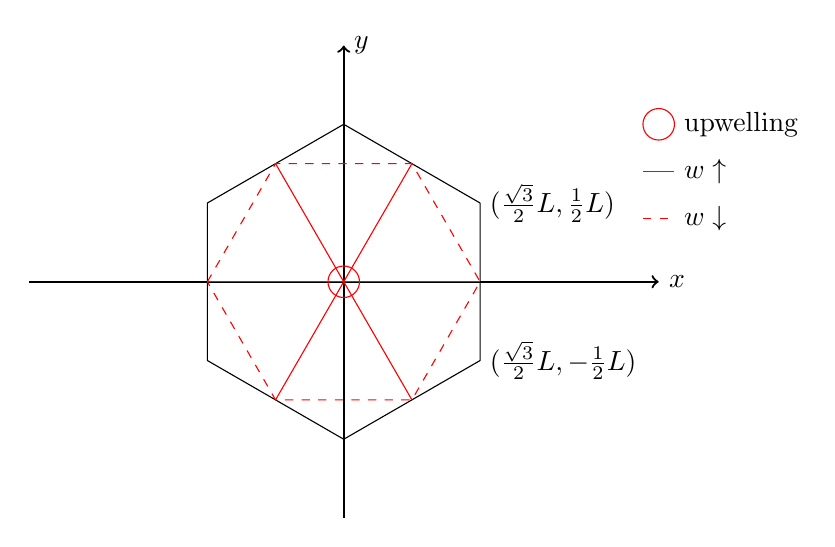
\begin{tikzpicture}[scale=2]
				\draw[thick,->] (-2, 0) -- (2,0) node[right] {$x$};
				\draw[thick,->] (0, -1.5) -- (0,1.5) node[right] {$y$};
				\draw[red] (0,0) circle (0.1);
				\draw (0.866, 0.5) -- (0, 1) -- (-0.866, 0.5) -- (-0.866,
				-0.5) -- (0, -1) -- (0.866, -0.5) -- (0.866, 0.5);
				\draw[red] (-0.433, -0.75) -- (0.433, 0.75);
				\draw[red] (0.433, -0.75) -- (-0.433, 0.75);
				\draw[red] (-0.866,0) -- (0.866, 0);

				\draw[red,dashed] (-0.866, 0) -- (-0.433, 0.75) -- (0.433,
				0.75) -- (0.866, 0) -- (0.433,-0.75) -- (-0.433, -0.75) --
				(-0.866,0);

				\draw (0.866, 0.5) node[right]
				{$(\frac{\sqrt{3}}{2}L,\frac{1}{2}L)$};
				\draw (0.866, -0.5) node[right]
				{$(\frac{\sqrt{3}}{2}L,-\frac{1}{2}L)$};

				\draw[red] (2, 1) circle (0.1);
				\draw (2.1, 1) node[right] {upwelling};
				\draw[red] (1.9, 0.7) -- (2.1, 0.7);
				\draw (2.1, 0.7) node[right] {$w \uparrow$};
				\draw[red,dashed] (1.9, 0.4) -- (2.1, 0.4);
				\draw (2.1, 0.4) node[right] {$w \downarrow$};
			\end{tikzpicture}
		\end{center}
\end{enumerate}

\section{Centrifugal instabilities}
Flows with curved streamlines can be unstable due to centrifugal effects.
\subsection{Rayleigh's criterion}
We will concentrate on axisymmetric flows. Consider an azimuthal flow 
\begin{equation}
	\u = u_\theta(r)\hat{\symbf{\theta}} = r \Omega(r)\hat{\symbf{\theta}}
\end{equation}
The inviscid, axisymmetric equations for a general flow $\u = u_r
\hat{\symbf{r}} + u_\theta \hat{\symbf{\theta}} + u_z \hat{\symbf{z}}$ are

\begin{align}
	\frac{\partial u_r}{\partial t} + \u \cdot \nabla u_r -
	\frac{u_\theta^2}{r} &= - \frac{1}{\rho}\frac{\partial p}{\partial r} \\
	\frac{\partial u_\theta}{\partial t} + \u \cdot \nabla u_\theta +
	\frac{u_r u_\theta}{r} &= - \cancel{\frac{1}{\rho}\frac{1}{r}\frac{\partial
p}{\partial \theta}} \\
	\frac{\partial u_z}{\partial t} + \u \cdot \nabla u_z
	 &= - \frac{1}{\rho}\frac{\partial p}{\partial z} \\
	 \frac{1}{r}\frac{\partial}{\partial r}(ru_r) +
	 \cancel{\frac{1}{r}\frac{\partial u_\theta}{\partial \theta}} +
			\frac{\partial u_z}{\partial z} &= 0 
\end{align}
where $\u \cdot \nabla = u_r \frac{\partial}{\partial r} + \cancel{
\frac{u_\theta}{r}\frac{\partial}{\partial \theta}} + u_z
\frac{\partial}{\partial z}$. Cancelled terms are absent in the axisymmetric
setting. The \emph{centrifugal} term is $-u_\theta^2/r$ in the $r$-momentum
equation. The $\theta$-momentum equation can be rearranged, and multiplied by
$r$ to give a material conservation equation:
\begin{align}
	\frac{\partial}{\partial r} (ru_\theta) + r u_r \frac{\partial
	u_\theta}{\partial r} + u_z \frac{\partial}{\partial z} (ru_\theta) +
	r\left(\frac{u_r u_\theta}{r}\right) &= 0 \\
	\implies \frac{\partial}{\partial t} (ru_\theta) + u_r
	\frac{\partial}{\partial r}(ru_\theta) + u_z \frac{\partial}{\partial
z}(ru_\theta) &= 0  \\
\implies \frac{\diffD}{\diffD t} (ru_\theta) &= 0
\end{align}

This expresses conservation of angular momentum: the angular momentum per unit
mass is $I = ru_\theta$, hence $\frac{\diffD I}{\diffD t} = 0$. This result
also follows from Kelvin's circulation theorem, using the circulation $\Gamma
= 2\pi r u_\theta$ for an inviscid fluid. The statement says that if $\u =
u_\theta(r)\hat{\symbf{\theta}}$ (i.e. axisymmetric azimuthal flow) then $I =
I(r)$ is a basic state.


\paragraph{What distributions of $I(r)$ could be stable?}
Rayleigh's argument considers 2 rings of fluid at radius $r_1$ and $r_2 (>
r_1)$ respectively. 
\begin{center}
	\begin{tikzpicture}
		\draw[thick,blue,->] (0,0) [partial ellipse=0:360:2 and .7];
		\draw[thick,blue,->] (0,0) [partial ellipse=0:360:2.5 and .9];
		\draw (0,0)  -- (2, 0) node[midway,below] {$r_1$};
		\draw (0,0)  -- (1.5, 0.72) node[midway,above] {$r_2$};
		\draw[thick,->] (0,0) -- (0, 1.5);
	\end{tikzpicture}
\end{center}

The kinetic energy is
\begin{equation}
	E = \frac{1}{2}\rho\left(\frac{I_1^2}{r_1^2} + \frac{I_2^2}{r_2^2}\right)
\end{equation}
Now suppose the rings swap places due to a perturbation, but they keep their
angular momentum (since it is materially conserved). The new KE is
\begin{equation}
	E_{\text{new}} = \frac{1}{2} \left( 
	\frac{I_2^2}{r_1^2} + \frac{I_1^2}{r_2^2}\right)
\end{equation}
Hence the swap has resulted in an energy change
\begin{equation}
	\Delta E = (I_2^2-I_1^2)\left(\frac{1}{r_1^2} - \frac{1}{r_2^2}\right)
\end{equation}
We can expect instability if $\Delta E < 0$. Since $r_2 > r_1$, the second
factor is positive hence
\begin{equation}
	\Delta E < 0 \iff I_2^2 < I_1^2
\end{equation}
Hence Rayleigh's criterion for stability is $I_2^2 \ge I_1^2$ or equivalently
\begin{equation}
	\frac{\diffd I^2}{\diffd r} \ge 0
\end{equation}
i.e. angular momentum does not increase outwards. Note that with $I =
ru_\theta = r^2 \Omega$ we have the condition
\begin{equation}
	\frac{\diffd}{\diffd r}\left( r^4 \Omega^2 \right) \ge 0
\end{equation}
for stability. This is often written using the \emph{Rayleigh determinant}
\begin{equation}
	\Phi \equiv \frac{1}{r}
	\frac{\diffd}{\diffd r}\left( r^4 \Omega^2 \right)
\end{equation}
Hence stability is predicted if $\Phi \ge 0$.

\subsection{Derivation via linear stability analysis}
Consider Taylor-Couette geometry: cylindrical walls at $r_1$ and $r_2$ with an
inviscid base state $\u = r \Omega(r) \hat{\symbf{\theta}}$, with axisymmetric
perturbations $\u'$. We have incompressibility
\begin{equation}
	\nabla \cdot \u' = 0 \implies \frac{1}{r}\frac{\partial}{\partial
	r}(ru_r') + \frac{\partial u_z'}{\partial z} = 0
\end{equation}
The Euler equations for this perturbation are
\begin{align}
	\frac{\partial u_r'}{\partial t} - \frac{2r \Omega u_\theta'}{r} &=
	-\frac{1}{\rho} \frac{\partial p'}{\partial r} \\
	\frac{\partial u_\theta'}{\partial t} + u_r'\frac{\diffd}{\diffd
r}(r\Omega) + \frac{u_r' r \Omega}{r} &= 0 \\
\frac{\partial u_z'}{\partial t} &= -\frac{1}{\rho}\frac{\partial p'}{\partial
z}
\end{align}
Now specify normal mode decomposition
\begin{equation}
	\begin{pmatrix} u_r' \\ u_\theta' \\ u_z' \\ p' \end{pmatrix} = 
	\begin{pmatrix} \hat{u}_r(r) \\ \hat{u}_\theta(r) \\ \hat{u}_z(r) \\
	\hat{p}(r) \end{pmatrix} e^{ikz + \sigma t}
\end{equation}
Only axisymmetric perturbations are considered. The Euler equations become
\begin{align}
	\frac{1}{r}\frac{\diffd}{\diffd r}(r\hat{u}_r) + ik \hat{u}_z &= 0 \\
	\sigma \hat{u}_r - 2\Omega \hat{u}_\theta &= - \frac{1}{\rho} \frac{\diffd
	\hat{p}}{\diffd r} \\
		\sigma \hat{u}_\theta + \hat{u}_r(\Omega + (r\Omega)_r) &= 0 \\
		\sigma \hat{u}_z &= -\frac{1}{\rho} ik \hat{p}
\end{align}
We can reduce this system down to a single equation for $\hat{u}_r$:
\begin{equation}
	\frac{\diffd}{\diffd r}\left(\frac{\diffd}{\diffd r} +
	\frac{1}{r}\right)\hat{u}_r - k^2 \hat{u}_r -2\frac{k^2}{\sigma^2}
	\Omega(2\Omega + r\Omega')\hat{u}_r = 0
\end{equation}
This is a second order ODE for $\hat{u}_r$ with BCs $\hat{u}_r = 0$ at $r=
r_1, r_2$. For this flow, Rayleigh's determinant is
\begin{equation}
	\Phi \equiv \frac{1}{r}
	\frac{\diffd}{\diffd r}\left( r^4 \Omega^2 \right) = 4\Omega^2 + 2r\Omega'
	\Omega
\end{equation}
Hence the ODE for $\hat{u}_r$ may be written as
\begin{equation}
	\frac{\diffd}{\diffd r}\left(\frac{1}{r}\frac{\diffd}{\diffd
	r}(r\hat{u}_r)\right) - k^2 \hat{u}_r = \frac{k^2}{\sigma^2} \Phi(r)
	\hat{u}_r
	\label{eq:l5}
\end{equation}
Multiply \eqref{eq:l5} by $r\hat{u}_r^*$ (complex conjugate) and integrate
from $r_1$ to $r_2$:
\begin{equation}
	\int_{r_1}^{r_2} r \hat{u}_r^* \frac{\diffd}{\diffd r} \left(
	\frac{1}{r}\frac{\diffd}{\diffd r}(r\hat{u}_r)\right) \diffd r - k^2
	\int_{r_1}^{r_2} r \abs{\hat{u}_r}^2 \, \diffd r = \frac{k^2}{\sigma^2}
	\int_{r_1}^{r_2} r \Phi \abs{\hat{u}_r}^2 \, \diffd r
\end{equation}
The first term may be integrated by parts to give:
\begin{equation}
	\cancel{\left[ r\hat{u}_r^* \frac{1}{r} \frac{\diffd}{\diffd
	r}(r\hat{u}_r)\right]_{r_1}^{r_2}}
	-\int_{r_1}^{r_2} \frac{\diffd}{\diffd r}(r \hat{u}_r^*)\frac{1}{r} \frac{\diffd}{\diffd r} (r\hat{u}_r) \diffd r - k^2
	\int_{r_1}^{r_2} r \abs{\hat{u}_r}^2 \, \diffd r = \frac{k^2}{\sigma^2}
	\int_{r_1}^{r_2} r \Phi \abs{\hat{u}_r}^2 \, \diffd r
\end{equation}
The first term vanishes since $\hat{u}_r =0$ at $r=r_1,r_2$. Labelling the
first integral as $H_1 > 0$ and the second as $H_2 > 0$, we have
\begin{equation}
	\frac{k^2}{\sigma^2}
	\int_{r_1}^{r_2} r \Phi \abs{\hat{u}_r}^2 \, \diffd r = -H_1 - k^2 H_2 < 0
\end{equation}
If $\Phi \ge 0$ then $\sigma^2 < 0$, i.e. $\sigma$ is imaginary and we have
stability. If instead $\Phi < 0$ somewhere in the domain, then potentially
\begin{equation}
	\int_{r_1}^{r_2} r \Phi \abs{\hat{u}_r}^2 \, \diffd r < 0
\end{equation}
in which case $\sigma^2 > 0$ and we have instability. Hence $\Phi < 0$
somewhere in the domain is \emph{necessary} (but not sufficient) condition for
instability. So this formal analysis confirms Rayleigh's heuristic criterion.
Note, really we need to consider non-axisymmetric perturbations too.

\subsection{Taylor vortices}
Apply Rayleigh's criterion to Taylor-Couette flow.
\begin{center}
	\begin{tikzpicture}
		\draw[thick,name path =A] (0,0) ellipse (1 and 0.2);
		\draw[thick,name path =B] (0,0) ellipse (1.5 and 0.4);
		\draw (0,-3) ellipse (1 and 0.2);
		\draw[thick] (0,-3) [partial ellipse = -180:0:1.5 and 0.4];
		\draw (0,-3) [partial ellipse = 0:180:1.5 and 0.4];
		\draw[->] (0,0) [partial ellipse = -10:60:1.6 and 0.5]
		node[midway,above] {$\Omega_2$};
		\draw[->] (0,0) [partial ellipse = -10:50:0.9 and 0.15]
		node[midway,left] {$\Omega_1$};
		\draw[thick] (1.5,0) -- (1.5, -3);
		\draw[thick] (-1.5, 0) -- (-1.5, -3);
		\draw (1, 0) -- (1, -3);
		\draw (-1, 0) -- (-1, -3);
		\draw[dashed] (0,1) -- (0, -3);
		\draw[<->] (0,-1.2) -- (1, -1.2) node[midway,above] {$R_1$};
		\draw[<->] (0,-2) -- (1.5, -2) node[midway,above] {$R_2$};
		\tikzfillbetween[of=A and B]{blue, opacity=0.2}
	\end{tikzpicture}
\end{center}

When viscosity is present, the general solution with $\partial_\theta =
\partial_z = 0$ is
\begin{equation}
	u_\theta(r) = A r + \frac{B}{r}
\end{equation}
No-slip boundary conditions at $r=R_1,R_2$ give
\begin{equation}
	A = \frac{\Omega_2 R_2^2 - \Omega_1 R_1^2}{R_2^2 - R_1^2}, \hspace{2em} B
	= \frac{\Omega_1 - \Omega_2}{R_1^{-2} - R_2^{-2}}
\end{equation}
Note this solves $(\nabla^2 - 1/r^2)u_\theta = 0$ where $\nabla^2 =
\frac{1}{r}\partial_r(r \partial_r)$. In this case $\Omega = u_\theta/r = A +
B/r^2$ hence Rayleigh's determinant is
\begin{equation}
	\Phi = \frac{1}{r^3} \frac{\diffd}{\diffd r}\left(r^4 \Omega^2\right) =
	\frac{1}{r^3} \frac{\diffd}{\diffd r} \left[ r^4 \left(A^2 + \frac{2AB}{r^2} +
	\frac{B^2}{r^4}\right)\right] = 4A^2\left(1+\frac{B}{Ar^2}\right)
\end{equation}
For convenience we define $\mu = \Omega_2/\Omega_1$ and $\eta = R_1 / R_2 <
1$. Then
\begin{equation}
	\Phi = 4A^2 \left[ 1 - \frac{(1-\mu)R_1^2}{(\eta^2 - \mu)r^2}\right]
\end{equation}
For stability, i.e. $\Phi \ge 0$ everywhere, we require for all $r \in \left[
R_1, R_2\right]$
\begin{equation}
	1 \ge \frac{(1-\mu)R_1^2}{(\eta^2 - \mu)r^2} \ge \frac{1-\mu}{\eta^2 -
	\mu}
\end{equation}
where the last inequality follows since $R_1^2 / r^2 \ge 1$ for all $r \in
\left[R_1, R_2\right]$. 
There are now two cases: 
\begin{itemize}
	\item If $\eta^2 > \mu$ then
	\begin{equation}
		\eta^2 - \mu \ge 1-\mu \implies \eta^2 \ge 1 
	\end{equation}
	This is a contradiction since $\eta < 1$. 
	\item Otherwise $\eta^2 < \mu$, so
	\begin{equation}
		\eta^2 - \mu \le 1 - \mu \implies \eta^2 \le 1
	\end{equation}
\end{itemize}
Thus Rayleigh's criterion is $\eta^2 < \mu$ for stability.

\begin{center}
	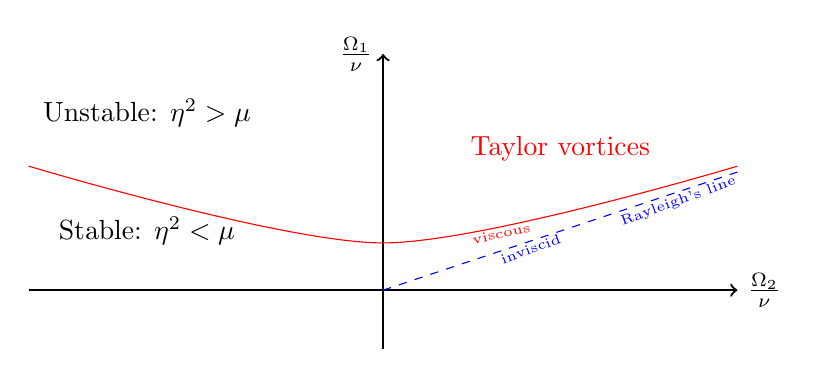
\begin{tikzpicture}[scale=1.5]
		\draw[thick,->] (-3,  0) --  (3, 0) node[right]
		{$\frac{\Omega_2}{\nu}$};
		\draw[thick,->] (0,  -0.5) --  (0, 2) node[left]
		{$\frac{\Omega_1}{\nu}$};
		\draw[dashed,blue] (0,0) -- (3, 1);
		\draw[red] plot[smooth] coordinates {(-3, 1.05) (0, 0.4) (3, 1.05)};
		\draw[red] (1, 0.48) node[rotate=12]{\tiny viscous};
		\draw[blue] (1.25, 0.35) node[rotate=20] {\tiny inviscid};
		\draw[blue] (2.5, 0.75) node[rotate=20] {\tiny Rayleigh's line};
		\draw (-2, 0.5) node {Stable: $\eta^2 < \mu$};
		\draw (-2, 1.5) node {Unstable: $\eta^2 > \mu$};
		\draw[red] (1.5, 1.2) node {Taylor vortices};
	\end{tikzpicture}
\end{center}

For a fixed geometry (i.e. fixed $\eta$) we can plot a stability diagram, with
Rayleigh's line $\eta^2 = \mu = \Omega_2 / \Omega_1$ marking the stability
heuristic. In Taylor-Couette geometry, the instability often manifests itself
as \emph{Taylor vortices}, though there are many different modes of
instability depending on $\Omega_1, \Omega_2, \nu$.

\begin{figure}
	\centering
	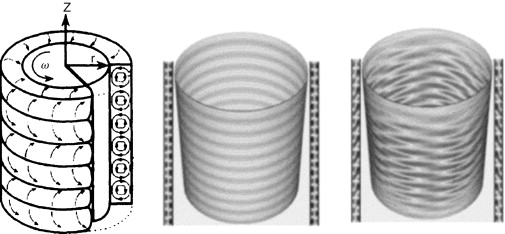
\includegraphics[width=0.5\textwidth]{taylor_vortices.jpg}
	\caption{Taylor vortices, from Dutta and Ray, 2004.}
\end{figure}

\section{Parallel shear flows}
For some flows, inviscid analysis gives a good approximation to the stability
properties of a viscous fluid (e.g. Kelvin-Helmholtz, Taylor-Couette flow) but
for others, it does not (e.g. plane Couette flow, channel flow, pipe  flow).
In these flows, viscosity can be \emph{de}stabilising.

\begin{center}
	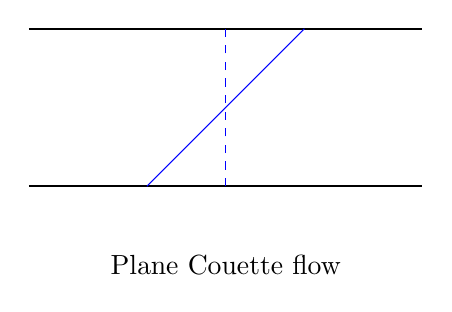
\begin{tikzpicture}
		\draw[thick] (0,0) -- (5, 0);
		\draw[thick] (0, 2) -- (5, 2);
		\draw[blue,dashed]  (2.5,0) -- (2.5, 2);
		\draw[blue] (1.5,0) -- (3.5, 2);
		\draw (2.5, -1) node {Plane Couette flow};
	\end{tikzpicture}
	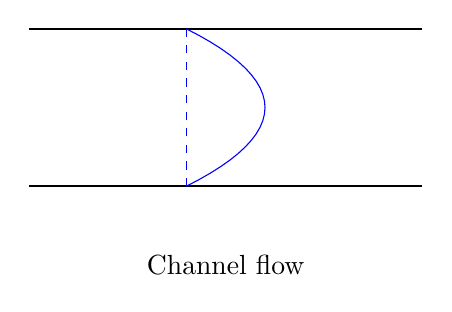
\begin{tikzpicture}
		\draw[thick] (0,0) -- (5, 0);
		\draw[thick] (0, 2) -- (5, 2);
		\draw[blue,dashed]  (2,0) -- (2, 2);
		\draw[blue] plot[domain=1:-1] ({3-\x*\x},{1+\x});
		\draw (2.5, -1) node {Channel flow};
	\end{tikzpicture}
	\begin{tikzpicture}
		\draw[thick] (1,0) -- (4, 0);
		\draw[thick] (1, 2) -- (4, 2);
		\draw[thick] (1, 1) [partial ellipse = -90:-270:0.5 and 1];
		\draw[thick] (4, 1) ellipse (0.5 and 1);
		\draw[blue,dashed]  (2,0) -- (2, 2);
		\draw[blue] plot[domain=1:-1] ({3-\x*\x},{1+\x});
		\draw (2.5, -1) node {Pipe flow};
	\end{tikzpicture}
\end{center}

\subsection{Inviscid analysis}
Consider a parallel shear flow $U(z)\hat{\symbf{x}}$. The non-dimensionalised
Euler equations are
\begin{align}
	\frac{\partial \u}{\partial t} + \u \cdot  \nabla \u &= - \nabla p \\
	\nabla \cdot \u &= 0
\end{align}
with boundary conditions $\u \cdot \hat{\symbf{z}} = 0$ at $z=z_1,z_2$. The
basic flow is $\symbf{U} = U(z)\hat{\symbf{x}}$ with $P$ constant -- any
constant form of the pressure is valid.  Add small perturbations
\begin{equation}
	\u = U(z)\hat{\symbf{x}} + \u', \hspace{1em}p = P + p'
\end{equation}
The Euler equations become
\begin{align}
	\frac{\partial \u'}{\partial t} + U\frac{\partial \u'}{\partial x} + w'
	\frac{\diffd U}{\diffd z} \hat{\symbf{x}} &= - \nabla p' \\
	\nabla \cdot \u' &= 0 
\end{align}
with boundary conditions $w' = 0$ at $z=z_1, z_2$. All equations have
coefficients independent of $x, y, t$ so we can separate the variables by
taking normal modes of the form
\begin{align}
	\u'(\x,t) &= \hat{\u}(z) e^{i(\alpha x  + \beta y - \alpha c t)} \\
	p'(\x,t)  &= \hat{p}(z) e^{i(\alpha x+ \beta y - \alpha c t)}
\end{align}
Note we have replaced the usual $\sigma$ with $-i\alpha c$. It is understood
that the physical fluid perturbation velocity $\u'$ is represented by the real
part, e.g.
\begin{equation}
	w' = \left[ \Re(\hat{w})\cos(\alpha x + \beta y - \alpha c_r t)
	-\Im(\hat{w})\sin(\alpha x+\beta y - \alpha c_r t)\right] e^{\alpha c_i t}
\end{equation}
This mode is a wave travelling with phase speed  $\alpha c_r /\sqrt{\alpha^2 +
\beta^2}$ in the $(\alpha, \beta, 0)$ direction and it decays like $e^{\alpha
c_i t}$ for $c_i < 0$, or grows if $c_i > 0$.  The equations are now
\begin{align}
i\alpha (U-c)\hat{u} + \frac{\diffd U}{\diffd z} \hat{w} + i \alpha\hat{p} &=
0 \label{eq:l6:1}\\
i\alpha (U-c)\hat{v} +  i \beta\hat{p} &=
0 \label{eq:l6:2} \\
i\alpha (U-c)\hat{w} +  \frac{\diffd \hat{p}}{\diffd z} &=
0 \label{eq:l6:3}\\
i\alpha \hat{u} + i\beta \hat{v} + \frac{\diffd \hat{w}}{\diffd z} &=
0\label{eq:l6:4}
\end{align}
with boundary conditions  $\hat{w}= 0$ at $z=z_1, z_2$. This is an eigenvalue
problem in $c \in \mathbb{C}$. Instability  corresponds to $c_i > 0$ and $c_i
\le 0$ for stability.

\subsubsection{Squire's transformation (Squire, 1933)}
Before  attempting to solve \eqref{eq:l6:1}--\eqref{eq:l6:4}, we consider
Squire's transformation. Define the transformed variables
\begin{equation}
	\tilde{\alpha} = \sqrt{\alpha^2 + \beta^2},\hspace{1em} \tilde{u} =
	\frac{\alpha \hat{u} + \beta \hat{v}}{\tilde{\alpha}}, \hspace{1em}
	\tilde{p} = \frac{\tilde{\alpha}\hat{p}}{\alpha}
\end{equation}
Construct $(\alpha\eqref{eq:l6:1} + \beta\eqref{eq:l6:2})/\alpha$:
\begin{equation}
	i\tilde{\alpha}(U-c)\tilde{u} + \frac{\diffd  U}{\diffd z} \hat{w} +
	i\tilde{\alpha}\tilde{p} =  0\label{eq:l6:5}
\end{equation}
Similarly $\tilde{\alpha}\eqref{eq:l6:3}/\alpha$:
\begin{equation}
	i\tilde{\alpha}(U-c)\hat{w} + \frac{\diffd \tilde{p}}{\diffd z} =
	0\label{eq:l6:6}
\end{equation}
Incompressibility is now expressed as
\begin{equation}
	i\tilde{\alpha}\tilde{u}  + \frac{\diffd \hat{w}}{\diffd z} = 0
\end{equation}

The transformed system has the same form as \eqref{eq:l6:1}--\eqref{eq:l6:4}
with $\beta = \hat{v} = 0$ and $\alpha \to \tilde{\alpha},
\hat{u}\to\tilde{u}, \hat{p}\to\tilde{p}$ but $c$ unchanged. Thus the
eigenvalue $c$ depends on $\sqrt{\alpha^2+\beta^2}$ but the growth rate is
$\alpha c_i$. So the largest growth rate $\alpha c_i$ is given by $\beta = 0$
for all wavenumber pairs $(\alpha,\beta)$ with $\sqrt{\alpha^2 + \beta^2}$
constant. Hence it is sufficient to consider $\beta = 0$ disturbances only. To
any unstable 3D mode $\alpha \ne 0, \beta \ne 0$ there corresponds a more
unstable 2D mode with $\beta = 0$.

\subsubsection{Rayleigh's equation}
Work in 2D (Squires). Use streamfunction $\psi'$ such that
\begin{equation}
	u' = \psi_z', \,\,v' = 0, \,\,w' = -\psi_x'
\end{equation}
Further, let $\psi'(x,z,t) = \phi(z)e^{i\alpha(x-ct)}$ so that it is  now
clear that $c_r$ is the phase speed in the $x$ direction. Now $\hat{u} =
\frac{\diffd \phi}{\diffd z}$ and $\hat{w} = -i\alpha \phi$ (notice the phase
difference). Then \eqref{eq:l6:5} becomes
\begin{align}
	i\alpha(U-c)\frac{\diffd \phi}{\diffd z} + \frac{\diffd U}{\diffd
	z}(-i\alpha \phi) + i\alpha \hat{p} &= 0\\
	\implies \hat{p}&= \frac{\diffd U}{\diffd z}\phi - (U-c)\frac{\diffd
	\phi}{\diffd z}
\end{align}
Substituting into \eqref{eq:l6:6} gives
\begin{align}
	i\alpha (U-c)(-i\alpha \phi) + \frac{\diffd}{\diffd z}\left[ \frac{\diffd
	U}{\diffd z}\phi - (U-c)\frac{\diffd \phi}{\diffd z}\right] &= 0 \\
	\implies (U-c)(\phi'' - \alpha^2 \phi) - U'' \phi &=0 \label{eq:rayleigh}
\end{align}
with boundary conditions $\phi = 0$ at $z=z_1, z_2$. This is \emph{Rayleigh's
equation (1880)}.
\paragraph{Comments.}
\begin{itemize}
	\item Rayleigh's equation involves $\alpha^2$ only so need only consider
		$\alpha > 0$.
	\item If $(\phi,c)$ solves the problem then so does $(\phi^*, c^*)$. So if
		there exists a growing mode, there  also exists a corresponding
		decaying mode. Hence stability means $c \in \mathbb{R}$ for all
		$\alpha$.
	\item A singularity  exists at $U(z_c) = c$ -- this is called a critical
		layer and only occurs when $c \in \mathbb{R}$. Critical layers are
		important in solving IVPs and relating Rayleigh's equation to its
		viscous analogue, the Orr-Sommerfield equation (see later).
	\item There are two types of eigensolution:
		\begin{itemize}
			\item Continuous  spectrum $c \in \left[ \min U, \max
				U\right]$ and $\phi$ has a discontinuous derivative at $z_c$.
				This type of solution is never unstable.
			\item Discrete spectrum of complex conjugate pairs. This solution
				can be unstable.
		\end{itemize}
\end{itemize}

\subsubsection{Properties of Rayleigh's equation.}
\paragraph{Inflection point criterion.}
Suppose $c_i > 0$, i.e. consider an unstable mode. Multiply Rayleigh's
equation by $\phi^*$ and integrate from $z_1$ to $z_2$:
\begin{equation}
	\int_{z_1}^{z_2} \left[\phi^* \phi'' - \alpha^2 \abs{\phi}^2 - \frac{U''}{U-c}
	\abs{\phi}^2 \right]\diffd z = 0
\end{equation}
Integrate the first term by parts and note $\phi = \phi^* = 0$ at $z_1$ and
$z_2$. Hence
\begin{equation}
	\int_{z_1}^{z_2} \left[\abs{\phi'}^2  + \alpha^2 \abs{\phi}^2 +
	\frac{U''}{U-c}\abs{\phi}^2 \right] \diffd z =0 \label{eq:ipc}
\end{equation}
Take imaginary part:
\begin{align}
	\Im \left[ \int_{z_1}^{z_2} \frac{U''(U-c^*)}{\abs{U-c}^2} \abs{\phi}^2
	 \diffd z \right]&= 0 \\
\implies
	-c_i\int_{z_1}^{z_2} \frac{U''}{\abs{U-c}^2} \abs{\phi}^2
	\diffd z &= 0
\end{align}
But $c_i > 0$ so we must have
\begin{equation}
\int_{z_1}^{z_2} \frac{U''}{\abs{U-c}^2} \abs{\phi}^2
	\diffd z  = 0
\end{equation}
Now $\abs{U-c}^2 > 0$ and $\abs{\phi}^2 > 0 $ so $U''$ must change sign
somewhere in $\left[z_1,z_2\right]$. Thus $U''=0$ at least once is a necessary
condition for inviscid instability, called the \emph{inflection point
criterion}.

\paragraph{Fj\o rtoft's condition.}
A stronger form of the inflection point criterion was obtained by Fj\o rtoft
(1950): given a monotonic mean velocity profile $U(z)$, a necessary condition
for instability is that $U''(U-U_s) < 0$ for some $z \in \left[ z_1, z_2
\right]$ with $U_s = U(z_s)$ where $U''(z_2) = 0$.

To see this, take the real part of \eqref{eq:ipc} to get
\begin{equation}
	\int_{z_1}^{z_2} \frac{U''(U-c_r)}{\abs{U-c}^2} \abs{\phi}^2 \, \diffd z =
	-\int_{z_1}^{z_2} \abs{\frac{\diffd \phi}{\diffd z}}^2 + \alpha^2
	\abs{\phi}^2 \, \diffd z
\end{equation}
Add the term
\begin{equation}
	(c_r - U_s)\int_{z_1}^{z_2} \frac{U''}{\abs{U-c}^2} \abs{\phi}^2
	\diffd z  = 0
\end{equation}
which vanishes if $c_i > 0$ by above. Then
\begin{equation}
	\int_{z_1}^{z_2} \frac{U''(U-U_s)}{\abs{U-c}^2} \abs{\phi}^2 \, \diffd z =
	-\int_{z_1}^{z_2} \abs{\frac{\diffd \phi}{\diffd z}}^2 + \alpha^2
	\abs{\phi}^2 \, \diffd z
\end{equation}

The RHS terms are negative definite, and $\abs{\phi^2} > 0$ as well as
$\abs{U-c}^2 > 0$. Hence $U''(U-U_s) < 0$ somewhere in $\left[z_1,z_2\right]$.
This means that the inflection point has to be a maximum (rather than a
minimum) of the spanwise vorticity $U'(z)\hat{\symbf{y}}$.

\begin{center}
	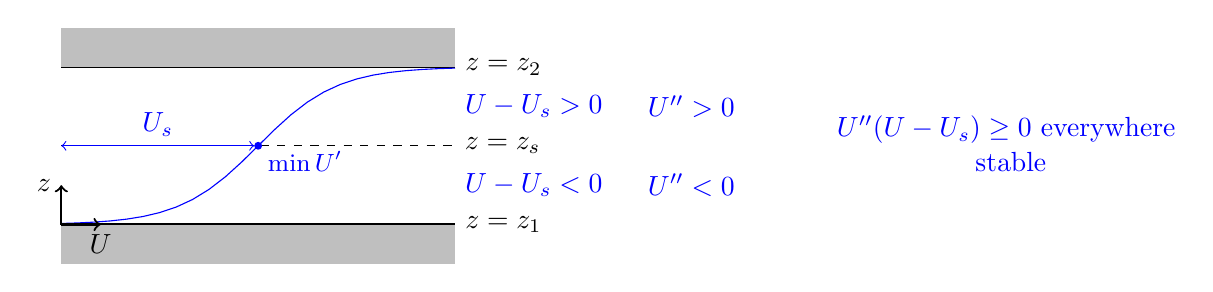
\begin{tikzpicture}
		\draw[thick] (0,0) -- (5, 0) node[right] {$z=z_1$};
		\draw[thick] (0, 2) -- (5, 2) node[right] {$z=z_2$};
		\draw[dashed] (0, 1) -- (5, 1) node[right] {$z=z_s$};
		\fill[gray!50] (0,0) rectangle (5, -0.5);
		\fill[gray!50] (0,2) rectangle (5, 2.5);
		\draw[blue] plot[domain=0:5] ({\x},{2/(1+e^(-2*(\x-2.5)))});
		\draw[blue] (2.5, 0.8) node[right] {\small $\min U'$};
		\draw[fill=blue,draw=none] (2.5, 1) circle (0.05);
		\draw[blue,<->] (0, 1) -- (2.5-0.05, 1) node[midway,above] {$U_s$};
		\draw[thick, ->] (0, 0) -- (0.5, 0) node[below] {$U$};
		\draw[thick, ->] (0, 0) -- (0, 0.5) node[left] {$z$};
		\draw[blue] (6, 1.5) node {$U - U_s > 0$};
		\draw[blue] (6, 0.5) node {$U - U_s < 0$};
		\draw[blue] (8, 1.5) node {$U'' > 0$};
		\draw[blue] (8, 0.5) node {$U'' < 0$};
		\draw[blue] (12, 1.2) node {$U''(U-U_s) \ge 0$ everywhere};
		\draw[blue] (12, 0.8) node {$\implies$ stable};
	\end{tikzpicture} \\
	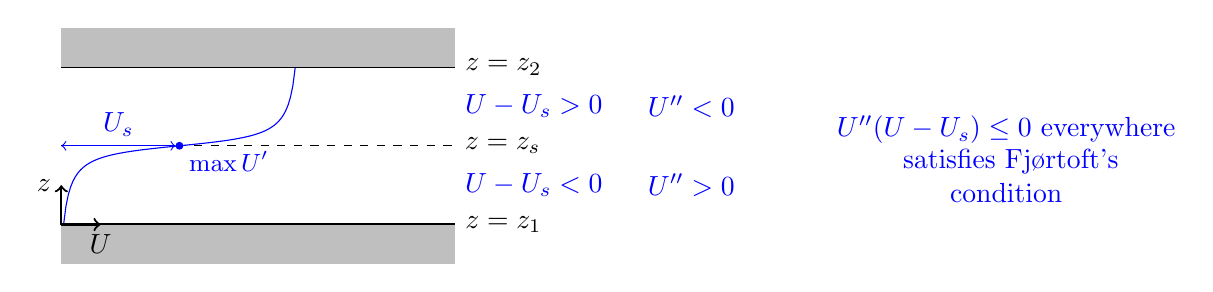
\begin{tikzpicture}
		\draw[thick] (0,0) -- (5, 0) node[right] {$z=z_1$};
		\draw[thick] (0, 2) -- (5, 2) node[right] {$z=z_2$};
		\draw[dashed] (0, 1) -- (5, 1) node[right] {$z=z_s$};
		\fill[gray!50] (0,0) rectangle (5, -0.5);
		\fill[gray!50] (0,2) rectangle (5, 2.5);
		\draw[blue] plot[domain=0.029:2.971,samples=100] ({\x},{1+ tan(deg(\x-1.5))/10});
		\draw[blue] (1.5, 0.8) node[right] {\small $\max U'$};
		\draw[fill=blue,draw=none] (1.5, 1) circle (0.05);
		\draw[blue,<->] (0, 1) -- (1.5-0.05, 1) node[midway,above] {$U_s$};
		\draw[thick, ->] (0, 0) -- (0.5, 0) node[below] {$U$};
		\draw[thick, ->] (0, 0) -- (0, 0.5) node[left] {$z$};
		\draw[blue] (6, 1.5) node {$U - U_s > 0$};
		\draw[blue] (6, 0.5) node {$U - U_s < 0$};
		\draw[blue] (8, 1.5) node {$U'' < 0$};
		\draw[blue] (8, 0.5) node {$U'' > 0$};
		\draw[blue] (12, 1.2) node {$U''(U-U_s) \le 0$ everywhere};
		\draw[blue] (12, 0.8) node {$\implies$ satisfies Fj\o rtoft's};
		\draw[blue] (12, 0.4) node {condition};
	\end{tikzpicture}
\end{center}

\paragraph{Howard's semicircle theorem}
Due to Howard (1961). The unstable eigenvalues of the Rayleigh equation
satisfy
\begin{equation}
	\left[ c_r - \frac{1}{2}(U_{\max} + U_{\min})\right]^2 + c_i^2 \le \left[
	\frac{1}{2}(U_{\max}-U_{\min})\right]^2
\end{equation}
This is best viewed as a geometric condition: the unstable eigenvalues lie in
a semicircle centred at $\frac{1}{2}(U_{\max}+U_{\min})$ of radius
$\frac{1}{2}(U_{\max}-U_{\min})$.
\begin{center}
	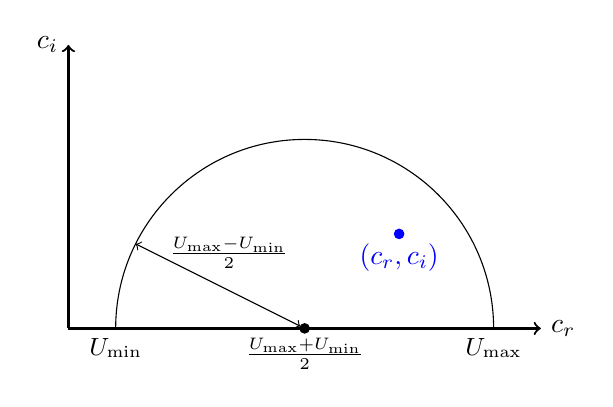
\begin{tikzpicture}[scale=1.2]
		\draw[thick,->] (0,0) -- (5, 0) node[right] {$c_r$};
		\draw[thick,->] (0,0) -- (0, 3) node[left] {$c_i$};
		\draw (0.5, 0) arc (180:0:2);
		\draw[fill] (2.5, 0) circle (0.05);
		\draw (0.5, 0) node[below] {\small $U_{\min}$};
		\draw (4.5, 0) node[below] {\small $U_{\max}$};
		\draw (2.5, 0) node[below] {\small $\frac{U_{\max}+U_{\min}}{2}$};
		\draw[<->] (2.455,0.0224) -- (0.711,0.8944);
		\draw (1.7,0.8) node {\small $\frac{U_{\max}-U_{\min}}{2}$};
		\draw[blue,fill] (3.5, 1) circle (0.05);
		\draw[blue] (3.5, 1) node[below] {$(c_r,c_i)$};
	\end{tikzpicture}
\end{center}

Let $\Psi = \frac{\phi}{U-c}$. Rayleigh's equation \eqref{eq:rayleigh} in
terms of $\Psi$ is
\begin{equation}
	(U-c)\left( \frac{\diffd^2}{\diffd z^2}\left[ (U-c)\Psi\right] - \alpha^2
	(U-c)\Psi\right) = U''(U-c)\Psi
\end{equation}
Evaluating the derivative and simplifying gives
\begin{equation}
	\frac{\diffd}{\diffd z}\left[ (U-c)^2 \frac{\diffd \Psi}{\diffd z}\right]
	= \alpha^2 (U-c)^2\Psi
\end{equation}
Multiply the equation by $\Psi^*$ and integrate over $\left[z_1,z_2\right]$:
\begin{equation}
	\int_{z_1}^{z_2} \Psi^*\left[(U-c)^2\Psi'\right]' \, \diffd z = \alpha^2
	\zint (U-c)^2 \abs{\Psi}^2 \, \diffd z
\end{equation}
We then integrate by parts and note that $\Psi = \phi/(U-c) = 0$ on $z=z_1,
z_2$. Hence
\begin{equation}
	\zint (U-c)^2 \left[ \abs{\Psi'}^2 + \alpha^2 \abs{\Psi}^2\right] \diffd z
	= 0
\end{equation}
Denote the $\left[\dots\right]$ factor by $Q$. We have $Q > 0$ and $c \in
\mathbb{C}$. Taking real and imaginary parts gives
\begin{align}
	\zint\left[ (U-c_r)^2 - c_i^2\right]Q \, \diffd z &= 0\\
	-2c_i\zint (U-c_r)Q \, \diffd z &= 0
\end{align}
Since $Q$ is strictly positive, $U-c_r$ has to change sign in
$\left[z_1,z_2\right]$. Hence 
\begin{equation}
	U_{\min} < c_r < U_{\max}
\end{equation}
Rewrite the imaginary part as
\begin{equation}
	\zint U Q \, \diffd z  = c_r \zint Q \, \diffd z
	\label{eq:l7:1}
\end{equation}
and the real part as
\begin{align}
	\zint U^2 Q \, \diffd z &\hspace{.3em}= 2 c_r \zint UQ \, \diffd z + (-c_r^2 + c_i^2)
	\zint Q \, \diffd z \\
							&\stackrel{\eqref{eq:l7:1}}{=} 2c_r^2 \zint Q \,
							\diffd z + (c_i^2 - c_r^2) \zint Q \, \diffd z \\
							&\hspace{.3em}= (c_r^2 + c_i^2) \zint Q \, \diffd
							z \label{eq:l7:2}
\end{align}

Now `notice' that
\begin{equation}
	\zint (U-U_{\min})(U-U_{\max})Q\, \diffd z \le 0
\end{equation}
since the first factor is $\ge 0$, the second is $\le 0$ and $Q > 0$.
Expanding the terms we have
\begin{equation}
	\zint \left[ U^2 Q - (U_{\min} + U_{\max}) UQ + U_{\min} U_{\max} Q
	\right]\diffd z \le 0
\end{equation}
Now using \eqref{eq:l7:1} and \eqref{eq:l7:2} we can rewrite as
\begin{align}
	\zint \left[ (c_r^2+c_i^2) - (U_{\min} + U_{\max})c_r +
	U_{\min}U_{\max}\right] Q \,\diffd z &\le 0 \\
	\implies \zint \left[ \left(c_r - \frac{U_{\max} + U_{\min}}{2}\right)^2  +
	 U_{\min}U_{\max} - \left(\frac{U_{\min}+U_{\max}}{2}\right)^2 +
	c_i^2\right] Q \,\diffd z &\le 0 \\
	\implies \zint \left[ \left(c_r - \frac{U_{\max} + U_{\min}}{2}\right)^2  +
	c_i^2 - \left(\frac{U_{\max}-U_{\min}}{2}\right)^2\right] Q \,\diffd z &\le 0
\end{align}
Equivalently we can write
\begin{equation}
	\left[ \left(c_r - \frac{U_{\max} + U_{\min}}{2}\right)^2  +
	c_i^2 - \left(\frac{U_{\max}-U_{\min}}{2}\right)^2\right] \zint Q \,\diffd
	z  \le 0
\end{equation}
But $\zint Q \, \diffd z > 0$ so
\begin{equation}
	\left(c_r - \frac{U_{\max} + U_{\min}}{2}\right)^2  +
	c_i^2 - \left(\frac{U_{\max}-U_{\min}}{2}\right)^2 \le 0
\end{equation}
which establishes the semicircle theorem.

\subsubsection{Predictions}
For channel flow $\symbf{U}(z) = (1-z^2)\hat{\symbf{x}}$ we have $U'' \ne 0$,
i.e. no inflection points, so no inviscid instability predicted. However,
channel flow is linearly unstable at sufficiently high Reynolds number. We
must add viscosity to gain a more accurate stability heuristic.

\subsection{Viscous analysis}
Consider a basic state $\symbf{U} = U(z)\hat{\symbf{x}}$ with $P = p_0 - Gx$
and $U(z_1) = U_-, U(z_2) = U_+$. At leading order, Navier-Stokes gives
\begin{equation}
	-G = \frac{1}{\ReN}U''
\end{equation}
\begin{center}
	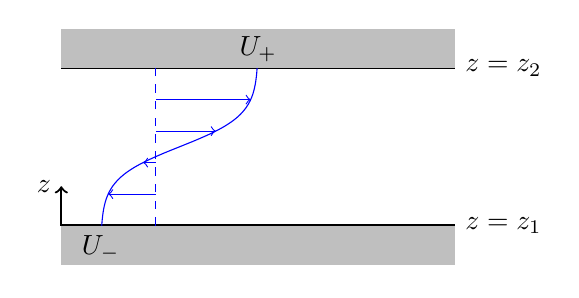
\begin{tikzpicture}
		\draw[thick] (0,0) -- (5, 0) node[right] {$z=z_1$};
		\draw[thick] (0, 2) -- (5, 2) node[right] {$z=z_2$};
		\fill[gray!50] (0,0) rectangle (5, -0.5);
		\fill[gray!50] (0,2) rectangle (5, 2.5);
		\draw[thick, ->] (0, 0) -- (0, 0.5) node[left] {$z$};
		\draw[blue,dashed] (1.2, 0) -- (1.2, 2);
		\draw[blue] plot[smooth,domain=0:2]
		({0.5+2/(1+e^(-5*(\x-1)))},	{\x});
		\draw[blue,->] (1.2, 0.4) -- (0.595, 0.4);
		\draw[blue,->] (1.2, 0.8) -- (1.038, 0.8);
		\draw[blue,->] (1.2, 1.2) -- (1.962, 1.2);
		\draw[blue,->] (1.2, 1.6) -- (2.405, 1.6);
		\draw (0.5, 0) node[below] {$U_-$};
		\draw (2.5, 1.95) node[above] {$U_+$};
	\end{tikzpicture}
\end{center}

Special cases are
\begin{itemize}
	\item Plane Poiseuille flow (PPF) $U(z) = 1-z^2$ in $\left[-1,1\right]$
		and $G = 2/\ReN$,$U_+ = U_- = 0$.
	\item Plane Couette flow (PCF) with $U(z) = z$ in $\left[-1,1\right]$ and
		$G = 0$, $U_+ = 1$, $U_- = -1$.
\end{itemize}
The linearised Navier-Stokes equations for a perturbation $\u', p'$ are
\begin{align}
	\frac{\partial u'}{\partial t} + U \frac{\partial u'}{\partial x} + w'
	\frac{\diffd U}{\diffd z} &= -\frac{\partial p'}{\partial x} +
	\frac{1}{\ReN} \nabla^2 u' \label{eq:l8:1}\\
	\frac{\partial v'}{\partial t} + U \frac{\partial v'}{\partial x}
							  &= -\frac{\partial p'}{\partial y} + 
							  \frac{1}{\ReN} \nabla^2 v' \label{eq:l8:2}\\
	\frac{\partial w'}{\partial t} + U \frac{\partial w'}{\partial x}
							  &= -\frac{\partial p'}{\partial z} + 
							  \frac{1}{\ReN} \nabla^2 w' \label{eq:l8:3} \\
	\frac{\partial u'}{\partial x} + \frac{\partial v'}{\partial y} +
	\frac{\partial w'}{\partial z} &= 0\label{eq:l8:4}
\end{align}

The divergence of the first three equations is
\begin{equation}
	\nabla \cdot \begin{pmatrix} \eqref{eq:l8:1} \\ \eqref{eq:l8:2} \\
	\eqref{eq:l8:3} \end{pmatrix} \implies \frac{\partial w'}{\partial x}
	\frac{\diffd U}{\diffd z} + \frac{\diffd U}{\diffd z} \frac{\partial
	w'}{\partial x} = -\nabla^2 p'
\end{equation}
Hence $\nabla^2 p' = -2 U' w'_x$. Now consider $\nabla^2 \eqref{eq:l8:3}$:
\begin{equation}
	\nabla^2 \left[ \frac{\partial w'}{\partial z} + U \frac{\partial
	w'}{\partial x} \right] = -\frac{\partial}{\partial z} \nabla^2 p' +
	\frac{1}{\ReN} \nabla^4 w' 
\end{equation}
Combining these results we have
\begin{align}
	\left[ \frac{\partial}{\partial t} + U\frac{\partial}{\partial x} -
	\frac{1}{\ReN} \nabla^2 \right] \nabla^2 w' + U'' \frac{\partial
	w'}{\partial x} + 2 \frac{\diffd U}{\diffd z} \frac{\partial^2
w'}{\partial x \partial z} &= -\frac{\partial}{\partial z}\left( -2
\frac{\diffd U}{\diffd z} \frac{\partial w'}{\partial x}\right) \\
\implies \left[ \left( \frac{\partial}{\partial t} + U\frac{\partial}{\partial x} -
\frac{1}{\ReN} \nabla^2\right)\nabla^2 - U''\frac{\partial}{\partial x}\right]
w' &= 0 \label{eq:l8:5}
\end{align}
with boundary conditions $w' = w'_z = 0$ on the boundaries. This is a fourth
order PDE with 4 boundary conditions, so $w'$ is fully determined. To close
the problem we need another equation: first define the \emph{normal vorticity}
\begin{equation}
	\eta' \equiv \hat{\symbf{z}}\cdot \nabla \times \u = \frac{\partial
	u'}{\partial y} - \frac{\partial v'}{\partial x}
\end{equation}
Now $\partial_y \eqref{eq:l8:1} - \partial_x \eqref{eq:l8:2}$ gives
\begin{align}
	\frac{\partial\eta'}{\partial t} + U\frac{\partial \eta'}{\partial x} +
	\frac{\diffd U}{\diffd z} \frac{\partial w'}{\partial y} &= \frac{1}{\ReN}
	\nabla^2 \eta' \\
	\implies \left[ \frac{\partial}{\partial t} + U\frac{\partial}{\partial x} -
	\frac{1}{\ReN} \nabla^2\right] \eta' = -\frac{\diffd U}{\diffd z}
	\frac{\partial w'}{\partial y} \label{eq:l8:6}
\end{align}
with boundary conditions $\eta' = 0$ on the boundaries since tangential
velocities vanish at the boundaries. We have reduced $(u',v',w',p') \to (w',
\eta')$. Given $w'$ and $\eta'$ determined from \eqref{eq:l8:5} and
\eqref{eq:l8:6}, we can generate $v', w', p'$ from
\begin{align}
	u'_x + v'_y &= -w'_z \\
	u'_y - v'_x &= \eta' \\
	\nabla^2 p' &= - 2U'w'_x
\end{align}

\subsubsection{Orr-Sommerfeld \& Squire Equations}
Introduce normal modes / wavelike disturbances / apply a Fourier transform:
\begin{equation}
	(w', \eta')(x,y,z,t) = (\hat{w}(z), \hat{\eta}(z)) e^{i(\alpha x+ \beta y
	- \alpha c t)}
\end{equation}
Let $k^2 = \alpha^2 + \beta^2$ be the total horizontal wavenumber. Then
\eqref{eq:l8:5} and \eqref{eq:l8:6} become
\begin{align}
	\left[ i\alpha (U-c)(D^2 -k^2) - i\alpha U'' -
	\frac{1}{\ReN}(D^2-k^2)^2\right]\hat{w} &= 0 \label{eq:l8:7} \\
	\left[ i\alpha (U-c) - \frac{1}{\ReN} (D^2 - k^2)\right] \hat{\eta} &=
	-i\beta U' \hat{w} \label{eq:l8:8}
\end{align}
where $D \equiv \frac{\diffd}{\diffd z}$ as usual. Equation~\eqref{eq:l8:7}
is the \emph{Orr-Sommerfeld equation} (Orr 1907, Sommerfeld 1908) and
equation~\eqref{eq:l8:8} is the Squire equation (Squire 1933).

\begin{itemize}
	\item The Orr-Sommerfeld (OS) equation is the viscous extension of the
		Rayleigh equation.
	\item System \eqref{eq:l8:7} and \eqref{eq:l8:8} has two types of
		solution:
		\begin{enumerate}
			\item OS modes $(\hat{w},\hat{\eta})$ where $\hat{w}$ solves
			\eqref{eq:l8:7} and $\hat{\eta}$ is the forced response in
			\eqref{eq:l8:8}.
		\item Squire modes $(0, \hat{\eta})$ which are always damped. Consider
			$\eqref{eq:l8:8}/(-i\alpha)$:
			\begin{equation}
				c \hat{\eta} = U \hat{\eta} + \frac{i}{\alpha \ReN}
				(D^2-k^2)\hat{\eta} 
			\end{equation}
			Multiply by $\hat{\eta}^*$:
			\begin{equation}
				c \abs{\hat{\eta}}^2 = U \abs{\hat{\eta}}^2 + \frac{i}{\alpha \ReN}
				\hat{\eta}^*(D^2-k^2)\hat{\eta} 
			\end{equation}
			Take the imaginary part and integrate over $\left[z_1,z_2\right]$:
			\begin{align}
				c_i \zint \abs{\hat{\eta}}^2 \, \diffd z 
				&= \frac{1}{\alpha
					\ReN} \zint \frac{i\hat{\eta}^*(D^2-k^2)\hat{\eta} - 
				(-i)\hat{\eta}(D^2-k^2)\hat{\eta}^*}{2i} \, \diffd z \\
				&= \frac{1}{\alpha \ReN}\zint \frac{1}{2}( 
				\hat{\eta}^*D^2\hat{\eta} + \hat{\eta} D^2
				\hat{\eta}^*) - k^2 \abs{\hat{\eta}}^2 \, \diffd z \\
				&= -\frac{1}{\alpha \ReN} \zint \abs{D \hat{\eta}}^2 + k^2
				\abs{\hat{\eta}}^2 \, \diffd z < 0
			\end{align}
			Thus $c_i < 0$ so solutions are damped. 			
		\end{enumerate}
		Hence we just need to consider  the OS equation to establish instability.
	\item Squire's theorem holds for the OS equation. The 3D version is
		\begin{equation}
			(U-c)(D^2 -k^2) \hat{w} - U'' \hat{w} - \frac{1}{i\alpha
			\ReN}(D^2-k^2)^2 \hat{w} = 0
		\end{equation}
		Compare with the 2D version
		\begin{equation}
			(U-c)(D^2 -\hat{\alpha}^2) \hat{w} - U'' \hat{w} -
			\frac{1}{i\hat{\alpha}\hat{\ReN}}(D^2-\hat{\alpha}^2)^2 \hat{w} = 0
		\end{equation}
		where $\hat{\alpha} = k^2 = \alpha^2 + \beta^2$ and
		\begin{equation}
			\hat{\ReN} = \frac{\alpha \ReN_{3D}}{\hat{\alpha}} =
			\frac{\alpha}{\sqrt{\alpha^2 + \beta^2}}\ReN_{3D} \le \ReN_{3D}
		\end{equation}
		Thus each 3D OS mode corresponds to a 2D OS mode at a \emph{lower}
		\ReN. Note this is a slightly different result from the inviscid case
		where 2D always had a larger growth rate. We can instead note that if
		the critical Reynolds number for linear stability is $\ReN_c$ then
		\begin{equation}
			\ReN_c = \min_{\alpha,\beta} \ReN_c(\alpha,\beta) = \min_{\alpha}
			\ReN_c(\alpha,0)
		\end{equation}
		where the first equality defines $\ReN_c$ and the second is Squire's
		theorem. This led to a focus on the 2D OS equation.
	\item What is the connection between Rayleigh and OS equations? 
		\begin{itemize}
			\item OS is non-singular and has a countably infinite number of
				eigenvalues and its eigenfunctions are complete (Scheisted
				1960). Note if the interval of flow is unbounded, there is a
				continuous spectrum of neutrally stable eigenfunctions in
				addition to the discrete spectrum (Herron 1987). 
			\item OS equation is fourth order whilst Rayleigh's equation is
				second order. 2 OS modes approximate Rayleigh modes, the other
				2 modes fix the boundary conditions at the walls (lots of work
				on this -- see Drazin \& Reid (1981)).
			\item Today it is absolutely routine to numerically solve the OS
				eigenvalue problem for $\ReN \le 10^7$. Very famous paper by
				Orszag (1971) used spectral methods as opposed to shooting
				techniques or finite difference to predict $\ReN_c$ in channel
				flow.
		\end{itemize}
\end{itemize}

\subsubsection{Channel flow (PPF)}
Thomas (1953) found $\ReN_c = 5780$ at $\alpha_c = 1.026$ using finite
differences (FD). Further FD estimates came from Nachtshen (1964) with
$(\ReN_c, \alpha_c) = (5767,1.02)$ and Grosch \& Salwen (1968) with $(\ReN_c,
\alpha_c) = (5750, 1.025)$. The accepted result now is from Orszag (1971) with
$\ReN_c = 5772.22$ at $\alpha_c = 1.02056$ using spectral methods.

Solving the Orrfield-Sommerfield equation with $\ReN = 7000, \alpha = 1, \beta
=0$ gives the following plot.

\begin{center}
	\begin{tikzpicture}
		\draw[thick,->] (0,0) -- (5, 0) node[right] {$c_r$};
		\draw[thick,->] (0,0) -- (0, 5) node[left] {$c_i$};
		\draw (0,0) node[below] {$0$};
		\draw (4.5,0) node[below] {$1$};
		\draw (0,0) node[left] {$-1$};
		\draw (0,4.5) node[left] {$0$};
		\draw (3, 0) node[below] {$2/3$};
		\draw[red,dashed] (4.5, 0) -- (4.5, 5);
		\draw[red,dashed] (0, 4.5) -- (5, 4.5);
		\draw[fill] (3.01, 0.2) circle (0.05);
		\draw[fill] (3, 0.6) circle (0.05);
		\draw[fill] (3.02, 1.1) circle (0.05);
		\draw[fill] (3, 1.4) circle (0.05);
		\draw[fill] (2.98, 1.9) circle (0.05);
		\draw[fill] (2.96, 2.3) circle (0.05);
		\draw[fill] (3, 2.6) circle (0.05);
		\draw[fill] (3.01, 3) circle (0.05);
		\draw[fill] (3.23, 3.21) circle (0.05);
		\draw[fill] (3.56, 3.53) circle (0.05);
		\draw[fill] (3.91, 3.94) circle (0.05);
		\draw[fill] (4.19, 4.21) circle (0.05);
		\draw[fill] (4.41, 4.43) circle (0.05);
		\draw[fill] (2.85, 3.16) circle (0.05);
		\draw[fill] (2.58, 3.41) circle (0.05);
		\draw[fill] (2.26, 3.75) circle (0.05);
		\draw[fill] (1.97, 4.01) circle (0.05);
		\draw[fill] (1.7, 4.27) circle (0.05);
		\draw[fill] (1.36, 4.63) circle (0.05);
		\draw[fill] (1.73, 4.08) circle (0.05);
		\draw[fill] (2.18, 3.87) circle (0.05);
		\draw[fill] (2.48, 3.39) circle (0.05);
		\draw[fill] (2.86, 3.16) circle (0.05);
		\draw[red] (1.5, 3.5) node {$A$};
		\draw[red] (3.8, 4.2) node {$P$};
		\draw[red] (3.5, 1.7) node {$S$};
	\end{tikzpicture}
\end{center}

Note the single unstable eigenvalue with $c_i > 0$.  The eigenvalues arise in
3 families, denoted $A$ for Airy, $P$ for Pekeris, and $S$ for Scheisted. 
\begin{itemize}
	\item $A$: $c_r \to 0$, wall modes, advected towards wall
	\item $P$: $c_r \to 1$, centre modes, advected towards centreline
	\item $S$: $c_r \approx 2/3$, identified by Mach (1976).
\end{itemize}

Note that a parabolic base state does not have an inflection point, but
\emph{does} have an unstable mode for large $\ReN$. Hence viscosity must be
destabilising. The unstable mode is called a Tollmien-Schlichting mode/wave
(Tollmien 1935, Schlichting 1933). Tollmien was the first to show the OS
equation has instability for non-inflection point profiles. 

However, as $\ReN \to \infty$ we are left with the Rayleigh equation and
stability, so somewhere in between they must match up. The stability diagram
for the OS equation with finite Reynolds number appears as follows:
\begin{center}
	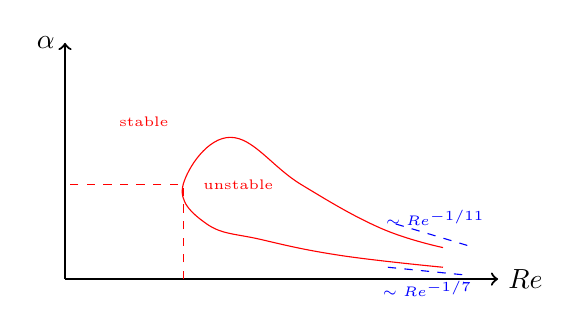
\begin{tikzpicture}
		\draw[thick,->] (0,0) -- (5.5, 0) node[right] {$\ReN$};
		\draw[thick,->] (0,0) -- (0, 3) node[left] {$\alpha$};
		\draw[red,dashed] (1.5, 0) -- (1.5, 1.2) -- (0, 1.2);
		\draw[red,smooth] plot[tension=0.7] coordinates {(4.8, 0.15) (3.5,
		0.3) (2.5, 0.5) (1.8, 0.7) (1.5, 1.2) (2.1, 1.8) (3, 1.2) (4, 0.65)
		(4.8, 0.4)};
		\draw[red] (2.2, 1.2) node {\tiny unstable};
		\draw[red] (1, 2) node {\tiny stable};
		\draw[blue,dashed] (4.2, 0.7) -- (5.2, 0.4) node[midway,above] {\tiny $\sim
		\ReN^{-1/11}$};
		\draw[blue,dashed] (4.1, 0.15) -- (5.1, 0.05) node[midway,below]
		{\tiny $\sim \ReN^{-1/7}$};
	\end{tikzpicture}
\end{center}

The neutral curve closes as there is no instability for $\ReN \to \infty$.

\subsubsection{Other flows}
\begin{table}[h]
	\begin{tabular}{c|ccccc}
		Type of flow & Profile & Stable? & $\ReN_{\text{crit}}$ &
		$\alpha_{\text{crit}}$ & Proof? \\ \hline
		Uniform & $U =$ const. & Yes & $\infty$ & -- & trivial \\
		PCF & $U = z, \,\,z \in \left[-1,1\right]$ & Yes & $\infty$ & -- &
		Romanov 1973 \\
		PPF & $U = 1-z^2,\,\, z \in \left[-1,1\right]$ & No & 5772 & 1.02 & --
		\\
		Blasius BL & $U = f'(z), z \ge 0$* & No & 520 & 0.3 & -- \\
		Shear layer & $U = \tanh z, -\infty < z < \infty$ & No & 0 & 0 & -- \\
		Jet/wake & $U = \sech^2 z, -\infty < z < \infty$ & No & 4.02 & 0.17 &
		-- \\
		HPF (pipe flow) & $\symbf{U} = (1-r^2)\hat{\symbf{z}},\,\, 0 < r < 1$
						& Yes & $\infty$ & -- & Chen et al., 2019?
	\end{tabular}
\end{table}

\paragraph{Notes.}
Blasius boundary layer (BL) profile $f$ solves $f''' + ff'' = 0$ subject to
$f(0) = f'(0) = 0, f'(\infty) = 1$. This is boundary layer flow over an
infinite plate. 

HPF stands for Hagen-Poiseuille flow. Pipe flow observed to be unstable at
$\ReN \approx \mathcal{O}(2000)$ (Reynolds, 1883). The transition is at
$\mathcal{O}(2000)$ with reasonable care, $\mathcal{O}(12,000)$ with a very
careful experiment to minimise disturbances. The world record is $\ReN \sim
10^5$ accredited to Pfenniger 1961.  Conclusion: pipe flow is unstable to
finite amplitude disturbances and threshold for instability \emph{decreases} as
$\ReN \to \infty$.

\section{Transient Growth \& IVPs}
So far in this course, the analysis has been `modal' -- identifying
eigenfunctions and eigenvalues of linear operators around basic states. This
can miss interesting features of the linearised dynamics over `short' times.
Need to consider initial value problems (IVPs).

\subsection{Example of IVP analysis}
\label{sec:eg}
Consider the initial value problem
\begin{align}
	\frac{\diffd}{\diffd t} \begin{pmatrix} v \\ \eta \end{pmatrix} &=
	\begin{pmatrix} -\frac{1}{\ReN} & 0 \\ 1 & -\frac{2}{\ReN} \end{pmatrix}
	\begin{pmatrix} v \\ \eta \end{pmatrix} + \begin{pmatrix} \eta^2 \\ -v\eta
\end{pmatrix}\label{eq:l9:1} \\
	&= \symsf{L}(\ReN) \begin{pmatrix} v \\ \eta \end{pmatrix} + \symbf{N}(v,
	\eta)
\end{align}
The first term is the linear part, and the second is the nonlinear part
emulating the nonlinearities of the dynamical equations. The eigenfunctions of
$\symsf{L}$ are $-1/\ReN$ and $-2/\ReN$ so a basic state
\begin{equation}
	\begin{pmatrix} v \\ \eta \end{pmatrix} = \symbf{0}
\end{equation}
is linearly stable. Then we must ask if all disturbances decay exponentially?
Certainly asymptotically ($t \to \infty$) \emph{but} not over short times. 

We can solve \eqref{eq:l9:1} linearised:
\begin{align}
	\dot{v} &= -\frac{1}{\ReN} v &&\implies v(t) = v_0 e^{-t/\ReN} \\
	\dot{\eta} &= v - \frac{2}{\ReN} \eta &&\implies (\eta e^{\frac{2t}{\ReN}})_t
			   = v_0 e^{t/\ReN} \\
			   & &&\implies \eta = \ReN v_0 e^{-t/\ReN} + (\eta_0 - \ReN
		v_0)e^{-2t/\ReN}
\end{align}
Hence the solution is
\begin{align}
	\begin{pmatrix} v \\ \eta \end{pmatrix} &= v_0 \begin{pmatrix} 1 \\ \ReN
	\end{pmatrix} e^{-t/\ReN} + (\eta_0 - \ReN v_0) \begin{pmatrix} 0 \\ 1
	\end{pmatrix} e^{-2t/\ReN} \\
	&= \begin{pmatrix} v_0\left(1-\frac{t}{\ReN}\right) + \mathcal{O}(t^2) \\
		\eta_0 + t\left(v_0 - \frac{2\eta_0}{\ReN}\right) + \mathcal{O}(t^2)
	\end{pmatrix}
\end{align}

The linearised solution demonstrates the possibility for short term
\emph{algebraic} growth of $\eta$ provided $v_0 - 2\eta_0/\ReN > 0$. To make
this more specific, define a norm
\begin{equation}
	E \equiv \frac{1}{2}\left(v^2 + \eta^2\right)
\end{equation}
and assume $\eta_0 = v_0 =1$. Then
\begin{align}
	E(t) &= \frac{1}{2}\left((1-t/\ReN + \dots)^2 + (1+t(1-2/\ReN) +
	\dots)^2\right) \\
		 &= 1 + \left(1-\frac{3}{\ReN}\right) t + \mathcal{O}(t^2)
\end{align}
So there is energy grwoth at least initially for $\ReN > 3$. What is going on?
The eigenvectors of $\symsf{L}$ are
\begin{align}
	(\lambda_1, \u_1) &= (-\frac{1}{\ReN},
	\frac{1}{\sqrt{1+\ReN^2}}\begin{pmatrix} 1 \\ \ReN \end{pmatrix} ) \\
	(\lambda_2, \u_2) &= (-\frac{2}{\ReN},
	\begin{pmatrix} 0 \\ 1\end{pmatrix} )
\end{align}
Note that these eigenvectors \emph{overlap}. They satisfy $\u_1^T \cdot \u_1 =
\u_2^T \cdot \u_2 = 1$ and also
\begin{equation}
	\u_1^T \cdot \u_2 = \frac{\ReN}{\sqrt{1+\ReN^2}} \to 1
	\,\,\,\text{as}\,\ReN \to \infty
\end{equation}
Hence the basis $\{\u_1,\u_2\}$ is very inefficient in representing
disturbances directed along $v$. For example,
\begin{equation}
	\begin{pmatrix} 1 \\ 0 \end{pmatrix} =
	\sqrt{1+\ReN^2}\u_1 - \ReN \u_2
\end{equation}
\begin{center}
	\begin{tikzpicture}
		\draw[thick,->] (0,0) -- (5, 0) node[right] {$v$};
		\draw[thick,->] (0,0) -- (0, 3) node[left] {$\eta$};
		\draw[blue,->] (0,0) -- (0, 2-0.05) node[midway,left] {$\u_2$};
		\draw[blue,->] (0,0) -- (0.82, 1.824) node[midway,right] {$\u_1$};
		\draw[blue,dashed] (0, 2) arc (90:0:2);
		\draw[blue] (0,2) node[left] {$\begin{pmatrix} 0 \\ 1 \end{pmatrix}$};
		\draw[blue,fill] (0,2) circle (0.05);
	\end{tikzpicture}
\end{center}

Since $\u_1$ and $\u_2$ decay at different rates, `growth' appears as large
coefficients $\sqrt{1+\ReN^2}, \ReN$ no longer largely cancel.

\subsection{Key points}
\paragraph{Matrix $L$ is non-normal.}
\begin{defn}
	A matrix $L$ is non-normal if $L^T L \ne L L^T$, otherwise $L$ is normal.
\end{defn}
Note this definition is extensible to operators, i.e. an operator $L$ is
normal if 
\begin{equation}
	\langle u, Lv \rangle = \langle L^T u, v \rangle \implies \langle u, L L^T
	v \rangle = \langle u, L^T L v\rangle
\end{equation}

For the matrix $L$ defined in \eqref{eq:l9:1}, we have
\begin{align}
	L^T L = 
	\begin{pmatrix}
		-\inv{\ReN} & 1 \\ 0 & -\frac{2}{\ReN} 
	\end{pmatrix}
	\begin{pmatrix}
		-\frac{1}{\ReN} & 0 \\ 1 & -\frac{2}{\ReN} 
	\end{pmatrix}
	&= \begin{pmatrix}
		-\frac{1}{\ReN^2} + 1 & -\frac{2}{\ReN} \\ -\frac{2}{\ReN} &
		\frac{4}{\ReN^2}
	\end{pmatrix} \\
	L L^T = 
	\begin{pmatrix}
		-\inv{\ReN} & 0 \\ 1 & -\frac{2}{\ReN} 
	\end{pmatrix}
	\begin{pmatrix}
		-\frac{1}{\ReN} & 1 \\ 0 & -\frac{2}{\ReN} 
	\end{pmatrix}
	&= \begin{pmatrix}
		\frac{1}{\ReN^2} & -\frac{1}{\ReN} \\ -\frac{1}{\ReN} &
		\frac{4}{\ReN^2} + 1
	\end{pmatrix}
\end{align}
So $L$ is non-normal.

\paragraph{Normality implies complete set of orthonormal eigenvectors.}
Hence a non-normal matrix has non-orthogonal eigenvectors. Consider all
complex square matrices $\mathbb{C}^{n \times n}$ and denote the Hermitian
conjugate by superscript $^H$. The space may be split into normal and
non-normal categories as follows.
\begin{center}
	\begin{tikzpicture}
		\draw (0,0) circle (1);
		\draw[name path = Aa, fill=red, opacity=0.2] (1,0) ellipse (2.5 and 1.5);
		\draw (1,0) ellipse (2.5 and 1.5);
		\draw (0.5,0) ellipse (3.5 and 2.5);
		\draw[name path = Bb] (-4, 3) rectangle (5, -3);
		\tikzfillbetween[of=Aa and Bb]{blue, opacity=0.2};
		\draw (0,0.5) node {$L = L^H$};
		\draw (0, 0) node {Hermitian};
		\draw (0, -0.4) node {adjoint};
		\draw[red] (2.1, 0.5) node {Normal};
		\draw[red] (2.1, 0.1) node {matrices};
		\draw[red] (2.1, -0.3) node {$LL^H = L^H L$};
		\draw (-1.5, -1.2) node[rotate=-30] {Diagonalisable};
		\draw (4.5, 2.5) node {$\mathbb{C}^{n\times n}$};
		\draw[blue] (-2, 2) node {Non-normal matrices};
		\draw[blue] (-2, 1.6) node {$LL^H \ne L^H L$};
		\draw (4, -2) node {Defective};
		\draw (4, -2.4) node {matrices};
		\draw (6, 0) node {$\begin{pmatrix} 1 & 1 \\ 0 & 1 \end{pmatrix}$};
		\draw[thick,->] (5.4, 0) -- (4, 1);
		\draw (-5, 0) node {$\begin{pmatrix} 1 & 1 \\ 0 & 2 \end{pmatrix}$};
		\draw[thick,->] (-4.6, 0) -- (-2, 0.5);
		\draw (-5.4, -1.7) node {$L$ from example};
		\draw[thick,->] (-5, -1.5) -- (-2.5, 0);
	\end{tikzpicture}
\end{center}

\paragraph{Choice of norm is important.}
Consider a general matrix $L$ which is diagonalisable, i.e. $\exists Q$ such
that $Q^{-1} L Q = \Lambda$, a diagonal matrix. Then there is no growth in the
norm 
\begin{equation}
	E' \equiv \x^T (Q^{-1})^T Q^{-1} \x = \x^T \symsf{W} \x
\end{equation}
where $\symsf{W} = (Q^{-1})^T Q^{-1}$ is the \emph{weight}.

\textbf{Proof:} let $\y = Q^{-1} \x$ and consider 
\begin{align}
	\frac{\diffd E'}{\diffd t} = \frac{\diffd}{\diffd t} \left( \y^T \cdot
	\y\right) = \y^T \cdot \dot{\y} + \dot{\y}^T \cdot \dot{\y} &= 2 \y^T
	\cdot \dot{\y} \\
			  &= 2 (Q^{-1}\x)^TQ^{-1}\dot{\x} \\
			  &= 2\x^T (Q^{-1})^T Q^{-1}\dot{\x} \\
			  &= 2 \x^T (Q^{-1})^T Q^{-1} \dot{\x} \\
			  &= 2 \x^T (Q^{-1})^T Q^{-1} L \x \hspace{2em} \text{since} \,\,
			  \dot{\x} = L \x \\
			  &= 2 \x^T (Q^{-1})^T Q^{-1} L Q Q^{-1} \x \\
			  &= 2 \x^T (Q^{-1})^T \Lambda Q^{-1} \x \\
			  &= 2 \y^T \Lambda \y 
\end{align}
Hence $\dot{E'}$ is negative if all eigenvalues of $\Re(\Lambda)$ are
negative. The key here is that $\y = Q^{-1} \x$ transforms $\x$ into a basis
of eigenvectors.  For example, for $L$ in the previous example we have
\begin{equation}
	Q = \begin{pmatrix} \frac{1}{\sqrt{1+\ReN^2}} & 0 \\
	\frac{\ReN}{\sqrt{1+\ReN^2}} & 1 \end{pmatrix} \implies Q^{-1} =
		\begin{pmatrix} \sqrt{1+\ReN^2} & 0 \\ -\ReN & 1 \end{pmatrix}
\end{equation}
Hence in the basis of eigenvectors $(v \,\,\, \eta)^T$ is
\begin{equation}
	Q^{-1}\x = Q^{-1} \begin{pmatrix} v \\ \eta \end{pmatrix} =
	\begin{pmatrix} v \sqrt{1+\ReN^2} \\ \eta - \ReN v \end{pmatrix}
\end{equation}
So above result indicates 
\begin{equation}
	(1+\ReN^2)_v^2 + (\eta- \ReN v)^2 = E'
\end{equation}
decays. We can calculate explicitly:
\begin{align}
	\frac{\diffd E'}{\diffd t} 
	&= 2(1+\ReN^2)v\dot{v} + 2(\eta-\ReN v)(\dot{\eta} - \ReN \dot{v}) \\
	&= 2 (1+\ReN^2)\left(\frac{-1}{\ReN^2} v^2\right) + 2(\eta - \ReN
	v)\left(2v - \frac{2\eta}{\ReN}\right) \\
	&= -\frac{2(1+\ReN^2)}{\ReN} v^2 - \frac{4(\eta - \ReN v)^2}{\ReN}\\
	&< 0 \,\,\, \text{for} \,\, v \ne 0, \eta \ne 0
\end{align}

\paragraph{Non-normality is necessary but not sufficient for transient
growth.}
Non-normality does not imply transient growth, but transient growth does imply
non-normality. For example, consider the norm $E$ defined in
section~\ref{sec:eg}, $E = (v^2 + \eta^2)/2$. We have
\begin{align}
	\dot{E} &= \left(v \,\,\,\, \eta\right) \begin{pmatrix} \dot{v} \\
	\dot{\eta} \end{pmatrix} \\
			&= -\frac{1}{\ReN} v^2 - \frac{2}{\ReN} \eta^2 + v \eta \\
			&= -\left(\frac{1}{\sqrt{\ReN}} v - \frac{\sqrt{\ReN}}{2} \eta
			\right)^2 + \left(\frac{\ReN^2 - 8}{4\ReN}\right) \eta^2
			\label{eq:l10:1}
\end{align}
So provided $\ReN^2 < 8$, no growth is possible even though $L$ is non-normal.
Note from \eqref{eq:l10:1} we can see that if $\ReN^2 > 8$ the maximum
\emph{initial} growth is obtained for $v_0 = \frac{\ReN}{2}\eta_0$ so if $E_0
=1$, then
\begin{equation}
	(v_0, \eta_0) = \left( \frac{\ReN\sqrt{2}}{\sqrt{4+\ReN^2}},
	\frac{\sqrt{8}}{\sqrt{4+\ReN^2}}\right)
\end{equation}
maximises the initial growth.

We can do the same analysis for the whole system
\begin{align}
	\dot{v} &= -\frac{1}{\ReN} v + \eta^2 \\
	\dot{\eta} &= v - \frac{2}{\ReN} \eta - v \eta
\end{align}
as the non-linearity is energy preserving (exactly as in the Navier-Stokes
equations). We have
\begin{equation}
	(v, \eta) \begin{pmatrix} \dot{v} \\ \dot{\eta} \end{pmatrix} 
	= (v, \eta) L \begin{pmatrix} v \\ \eta \end{pmatrix}
\end{equation}
as before. Thus the nonlinear terms satisfy
\begin{equation}
	(v, \eta) N(v, \eta) = 0 = v(\eta^2) + \eta(-v\eta)
\end{equation}
Hence \emph{any} initial condition will decay monotonically for $\ReN <
\sqrt{8}$, i.e. $(v, \eta) = \symbf{0}$ is then a global attractor.

Exactly the same type of analysis (energy stability analysis) can be done for
the Navier-Stokes equations (hope to revisit later).

\paragraph{How to find max growth and optimal ICs.}
We can find the optimal initial conditions as a function of $T$, a chosen
time. We have
\begin{equation}
	\frac{\diffd}{\diffd t}\begin{pmatrix} v \\ \eta \end{pmatrix} = L
	\begin{pmatrix} v \\ \eta \end{pmatrix} \implies \begin{pmatrix} v \\ \eta
	\end{pmatrix} = e^{Lt} \begin{pmatrix} v_0 \\ \eta_0 \end{pmatrix}
\end{equation}
Let $A \equiv e^{Lt}$. By direct calculation, we have
\begin{equation}
	A = \begin{pmatrix} e^{-t/\ReN} & 0 \\ \ReN(e^{-t/\ReN} - e^{-2t/\ReN}) &
	e^{-2t/\ReN} \end{pmatrix}
\end{equation}
or more generally
\begin{equation}
	e^{\begin{pmatrix} \lambda_1 & 0 \\ 1 & \lambda_2\end{pmatrix}t} =
	\sum_{n=0}^\infty \frac{1}{n!} \begin{pmatrix} \lambda_1 & 0 \\ 1 &
		\lambda_2 \end{pmatrix}^n t^n = \begin{pmatrix} e^{\lambda_1 t} & 0 \\
		\frac{e^{\lambda_1 t} - e^{\lambda_2 t}}{\lambda_1 - \lambda_2} &
		e^{\lambda_2 t} \end{pmatrix}
\end{equation}
Define the \emph{energy gain} at time $T$
\begin{align}
	G(T; \ReN) &\equiv \max_{v_0, \eta_0} \frac{E(T)}{E(0)} \\
			   &= \max_{v_0, \eta_0} \frac{(v(T) \,\,\,
				   \eta(T))\begin{pmatrix}v(T) \\ \eta(T) \end{pmatrix}}{(v_0
			   \,\,\, \eta_0) \begin{pmatrix} v_0 \\ \eta_0 \end{pmatrix}} \\
			   &= \max_{v_0, \eta_0} \frac{ \left[ A(T) \begin{pmatrix} v_0 \\
					   \eta_0 \end{pmatrix} \right]^T \left[ A(T)
					   \begin{pmatrix} v_0 \\ \eta_0 \end{pmatrix} \right]
					   }{(v_0 \,\,\, \eta_0)\begin{pmatrix} v_0 \\ \eta_0
\end{pmatrix}} \\
&= \max_{v_0, \eta_0} \frac{(v_0 \,\,\, \eta_0)A^T A \begin{pmatrix} v_0 \\
		\eta_0 \end{pmatrix}}{(v_0 \,\,\, \eta_0)\begin{pmatrix} v_0 \\ \eta_0
\end{pmatrix}}\\
&= \left\Vert A \right\Vert_2^2
\end{align}

The maximum over $v_0, \eta_0$ is equivalent to the maximum eigenvalue of $A^T
A$. Since $A^T A$ is real and symmetric, it is normal, so all eigenvalues are
real. $A^TA$ is also positive definite, so all eigenvalues are positive. The
norm
\begin{equation}
	\left\Vert A \right\Vert_2^2
\end{equation}
is usually computed using singular value decomposition (SVD). From the above,
we have
\begin{equation}
	G = \sigma_1^2 = \text{largest eigenvalue of}\,\, A^T A
\end{equation}
and $\sigma_1$ is the largest singular value of $A$. The corresponding
eigenvector is the optimal initial condition.

\subsection{Singular value decomposition}
In the previous section we refer to singular value decomposition; here we
demonstrate existence and uniqueness of SVD.

\paragraph{Theorem.}
Every matrix $A \in \mathbb{C}^{m \times n}$ has a SVD
\begin{equation}
	A = U \Sigma V^H
\end{equation}
where $U \in \mathbb{C}^{m \times m}$ and $V \in \mathbb{C}^{n \times n}$ are
unitary and $\Sigma = \text{diag}(\sigma_i) \in \mathbb{R}^{m \times n}$ with
$\sigma_1 < \sigma_2 < \dots$.  Furthermore, the singular values
$\{\sigma_j\}$ are uniquely determined and if $A$ is square ($m=n$) and the
$\sigma_j$ are distinct then the left and right singular vectors $\{u_j\}$,
$\{v_j\}$ are uniquely determined up to complex signs. Note in particular that
$\sigma_j \in \mathbb{R}$.

How can we relate eigenvalues of $A^T A$ to the singular values of $A$? Given
$A = U \Sigma V^H$ where $U^H U = I, V^H V = I$ and $\Sigma$ is diagonal, we
have
\begin{equation}
	AV = U\Sigma
\end{equation}
so $A$ maps columns of $V$ onto columns of $U$ with `scale' factors in
$\Sigma$, i.e. the singular values. For example,
\begin{equation}
	A\symbf{v}_i = \sigma_i \symbf{u}_i
\end{equation}
Similarly, $A^T = V \Sigma U^H$ so $A^T U = V \Sigma$ and $A^T$ maps columns
of $U$ back to columns of $V$, e.g. $A^T \symbf{u}_i = \sigma_i \symbf{v}_i$.
Hence
\begin{align}
	\sigma_i \symbf{v}_i = A^T \symbf{u}_i &= A^T \left(\frac{1}{\sigma_1} A
		\symbf{v}_i\right) \\
	\implies A^T A \symbf{v}_i &= \sigma_i^2 \symbf{v}_i
\end{align}

Thus $\sigma_i^2$ are eigenvalues of $A^T A$. Since $\sigma_i$ are ordered so
that $\sigma_1 > \sigma_2 > \dots$, $G = \sigma_1^2$ is the square of the
largest singular value of $A$.  

Note if $A$ is normal then singular values are eigenvalues. If $A$ is
non-normal, this does not hold.

\subsection{Energy growth in viscous channel flows}
This section is largely based on research work by Reddy \& Henningson, JFM,
\textbf{252}, pp. 209--238 (1993). Consider pressure driven flow through a
channel.

\begin{center}
	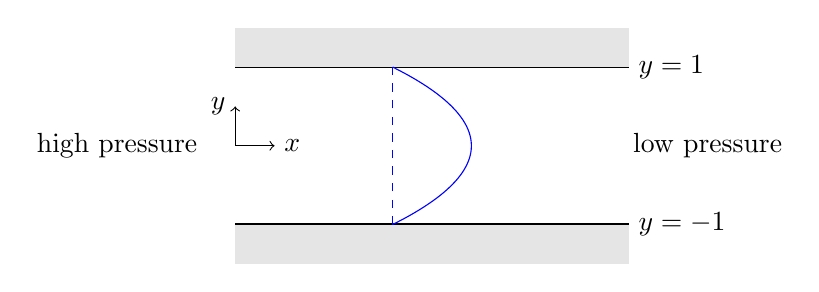
\begin{tikzpicture}
		\draw[thick] (0,0) -- (5, 0);
		\draw[draw=none,fill=gray!20] (0,0) rectangle (5, -0.5);
		\draw[thick] (0,2) -- (5, 2);
		\draw[draw=none,fill=gray!20] (0,2) rectangle (5, 2.5);
		\draw[blue,dashed] (2,0) -- (2,2);
		\draw[blue, smooth] plot[domain=-1:1] ({3-\x*\x},{1+\x});
		\draw (6, 1) node {low pressure};
		\draw (-1.5, 1) node {high pressure};
		\draw (5,2) node[right] {$y=1$};
		\draw (5,0) node[right] {$y=-1$};
		\draw[->] (0, 1) -- (0.5,1) node[right] {$x$};
		\draw[->] (0, 1) -- (0, 1.5) node[left] {$y$};
	\end{tikzpicture}
\end{center}

The basic state is $\symbf{U} = U(y)\symbf{\hat{x}}$ with $U(y) = 1-y^2$ and
$\nabla P = -\frac{2}{\ReN}\hat{\symbf{x}}$. Consider a perturbation $(\u,
p)$:
\begin{align}
	\symbf{u}_{\text{total}} &= U(y)\hat{\symbf{x}} + \u \\
	p_{\text{total}} &= P + p 
\end{align}

The linearised Navier-Stokes are (as usual)
\begin{align}
	\frac{\partial \u}{\partial t} + \u \cdot \nabla \symbf{U} +
	\symbf{U} \cdot \nabla \hat{\u} + \nabla p &= \frac{1}{\text{Re}} \nabla^2
	\u \label{eq:l11:1}\\
	\nabla \cdot \u &= 0
\end{align}

First, consider $\hat{\symbf{y}} \cdot \nabla \times \eqref{eq:l11:1}$:
\begin{equation}
	\left(\frac{\partial}{\partial t} + U \frac{\partial}{\partial x}\right)
	\eta + \frac{\partial v}{\partial z} \frac{\diffd U}{\diffd y} =
	\frac{1}{\ReN} \nabla^2 \eta
\end{equation}
where $\eta = \symbf{\hat{y}} \cdot \nabla \times \u = \partial_z u -
\partial_x w$ (using $\u = (u, v, w)$ as usual). Consider also
$\hat{\symbf{y}} \cdot \nabla \times (\nabla \times \eqref{eq:l11:1})$ which
gives
\begin{equation}
	\left(\frac{\partial}{\partial t} + U \frac{\partial}{\partial x}\right)
	\nabla^2 v - \frac{\partial v}{\partial x} \frac{\diffd^2 U}{\diffd y^2} =
		\frac{1}{\ReN} \nabla^4 v
\end{equation}
The no-slip boundary conditions $u = v = w = 0$ on $y = \pm 1$ translates to
BCs on $\eta$ and $v$:
\begin{align}
	\eta(y=\pm 1) &= 0 \\
	v(y=\pm 1) &= 0 \\
	\left.\frac{\partial v}{\partial y}\right|_{y=\pm 1} &= 0
\end{align}
where the last condition follows from $\nabla \cdot \u = 0$ and the fact
tangential derivatives also vanish on $y = \pm 1$. We have reduced the second
order system for 3 variables $(u, v, w)$ supplemented by $\nabla \cdot \u$ and
$p$ into a second and fourth order system for $v$ and $\eta$. 

We now take a Fourier transform in $x$ and $z$, i.e. write
\begin{equation}
	\left[ v(\x,t), \eta(\x,t)\right] = \left[ \hat{v}(y,t),
	\hat{\eta}(y,t)\right] e^{i(\alpha x + \beta z)}
\end{equation}
Then write
\begin{equation}
	\frac{\partial}{\partial t} \begin{pmatrix} \hat{v} \\ \hat{\eta}
		\end{pmatrix} = \begin{pmatrix} \L_{os} & 0 \\ \L_c & \L_{sq}
		\end{pmatrix} \begin{pmatrix} \hat{v} \\ \hat{\eta} \end{pmatrix} = \L
		\begin{pmatrix} \hat{v} \\ \hat{\eta}\end{pmatrix} \label{eq:l11:2}
\end{equation}
where
\begin{align}
	\L_{os} &= \frac{1}{D^2 -k^2} \left[ \frac{1}{\ReN} (D^2-k^2)^2 - i\alpha
	U (D^2-k^2) + i \alpha D^2 U\right] \\
	\L_c &= -i\beta D U \\
	\L_{sq} &= \frac{1}{\ReN} (D^2 - k^2) - i\alpha U
\end{align}
with $D \equiv \diffd/\diffd y$ and $k^2 = \alpha^2 + \beta^2$. The operators
$\L_{os}$ and $\L_c$ are the Orr-Sommerfeld (Orr 1907 \& Sommerfeld 1908) and
Squire (Squire 1933) operators, and $\L_c$ is the coupling operator. Notice
that the structure of \eqref{eq:l11:2} is reminiscent of the introductory
model in section~\ref{sec:eg}. 

We can write the solution to the IVP \eqref{eq:l11:2} in terms of an
eigenfunction expansion since they form a complete set (Diprima \& Habetler
1969) using the norm \eqref{eq:norm} defined later. Let $\{\lambda_j\}$
and $\{\mu_j\}$ be the eigenvalues of $\L_{os}$ and $\L_{sq}$ respectively.
Then
\begin{equation}
	\hat{\symbf{v}} = \begin{pmatrix} \hat{v}(y,t) \\ \hat{\eta}(y,t)
		\end{pmatrix} = \sum_j A_j e^{\lambda_j t} \begin{pmatrix}
	\tilde{v}_j(y) \\ \tilde{\eta}_j^p(y) \end{pmatrix} + \sum_j B_j e^{\mu_j
	t} \begin{pmatrix} 0 \\ \tilde{\eta}_j(y) \end{pmatrix} \label{eq:l11:3}
\end{equation}
The first sum is of OS modes, where $\{\tilde{v}_j\}$ are the
eigenfunctions of $\L_{os}$, and $\{\tilde{\eta}_j^p\}$ are the forced normal
vorticity ($\eta$) functions corresponding to the velocity functions. The
second sum is of Squire modes, where $\{\tilde{\eta}_j\}$ are the
eigenfunctions of $\L_{sq}$. The coefficients $\{A_j\}$ and $\{B_j\}$ are set
by the initial conditions.

We now combine the eigenvalues $\lambda_j$ and $\mu_j$ into a set
\begin{equation}
	\Lambda = \{ \lambda_j, \mu_j\}
\end{equation}
with $\Lambda_j$ ordered by decreasing real part. Further, define the
corresponding eigenfunctions to $\Lambda_j$ as
\begin{equation}
	\symbf{\tilde{q}}_j(y) = \begin{pmatrix} \tilde{v}_j(y) \\
	\tilde{\eta}_j(y) \end{pmatrix}
\end{equation}
The solution may then be written
\begin{equation}
	\hat{\symbf{v}}(y,t) = \sum_j a_j \symbf{\tilde{q}}_j(y) e^{\Lambda_j t}
	\label{eq:l11:4}
\end{equation}

Typically, we use the (kinetic) energy norm $E = \iint_{\alpha,\beta}
E(\alpha, \beta) \diffd \alpha \diffd \beta$ where
\begin{equation}
	E(\alpha,\beta) = \frac{1}{2}\int_{-1}^1 \{ \abs{\hat{u}}^2 +
	\abs{\hat{v}}^2 + \abs{\hat{w}}^2 \} \diffd y
\end{equation}

To determine $u$ and $w$ in terms of $v$ and $\eta$, consider $\eta = u_z -
w_x = i\beta u - i\alpha w$. Hence
\begin{equation}
	\nabla \cdot \u = 0 \implies -D v = i\alpha u + i\beta w
\end{equation}
In matrix form we have
\begin{equation}
	\begin{pmatrix} 
		i\alpha & i\beta \\ i\beta & -i\alpha \end{pmatrix} \begin{pmatrix} u
		\\ w \end{pmatrix} = \begin{pmatrix} -D v \\ \eta \end{pmatrix}
\end{equation}
Finally, inverting this equation gives
\begin{equation}
	\begin{pmatrix} u \\ w \end{pmatrix} = \frac{1}{k^2}\begin{pmatrix}
	-i\alpha & -i\beta \\ -i\beta & i\alpha \end{pmatrix} \begin{pmatrix} -Dv
	\\ \eta \end{pmatrix}
\end{equation}
Hence $u$ and $w$ can be written
\begin{align}
	u &= \frac{i\alpha Dv - i\beta \eta}{k^2} \\
	w &= \frac{i\beta Dv + i\alpha \eta}{k^2}
\end{align}
The energy norm may then be written as
\begin{equation}
	E(\alpha, \beta) = \norm{\symbf{\hat{v}}}^2= \frac{1}{2k^2} \int_{-1}^1
	\abs{D \hat{v}}^2 + k^2 \abs{\hat{v}}^2 + \abs{\hat{\eta}}^2 \, \diffd y
	\label{eq:norm}
\end{equation}

We now wish to determine the energy growth gain, defined by
\begin{equation}
	G(\alpha, \beta; \ReN, t) = \sup_{\symbf{\hat{v}}(y,0)}
	\frac{\norm{\hat{\symbf{v}}(y,t)}^2}{\norm{\hat{\symbf{v}}(y,0)}^2}
\end{equation}

Using the solution \eqref{eq:l11:4} (from \eqref{eq:l11:3}) derived above, we
have (note that supremum is now equivalently taken over initial condition
coefficients $\symbf{a}$)
\begin{align}
	G &= \sup_{\symbf{a}} \frac{ \norm{ \sum_j a_j \tilde{\symbf{q}}_j
	e^{\Lambda_j t}}^2 }{ \norm{ \sum_j a_j \tilde{\symbf{q}}_j}^2 } \\
	  &= \sup_{\symbf{a}} \frac{ \sum_i^N \sum_j^N a_i^* e^{\Lambda_i^* t}
		  \langle \tilde{\symbf{q}}_i, \tilde{\symbf{q}}_j \rangle a_j
	  e^{\Lambda_j t}}{ \sum_i^N \sum_j^N a_i^*
  \langle \tilde{\symbf{q}}_i, \tilde{\symbf{q}}_j \rangle a_j} \\
\end{align}
where $\langle\cdot,\cdot\rangle$ is the inner product
\begin{equation}
	\langle \tilde{\symbf{q}}_j, \tilde{\symbf{q}}_l\rangle = \frac{1}{2k^2}
	\int_{-1}^1 (D \hat{v}_j)^* D\hat{v}_l + k^2 \hat{v}_j^* \hat{v}_l +
	\hat{\eta}_j^* \hat{\eta}_l \, \diffd y
\end{equation}
Let $A_{ij} = \langle \tilde{\symbf{q}}_i, \tilde{\symbf{q}}_l\rangle$. Then
$A \in \mathbb{C}^{N \times N}$ is Hermitian ($A_{ij}^* = A_{ji}$) and
positive definite (the norm is positive definite). Then there exists a matrix
$F$ such that $A = F^H F$ (Cholesky decomposition). Using the notation
\begin{equation}
	e^{\Lambda t} = \text{diag}(e^{\Lambda_1 t}, e^{\Lambda_2 t}, \dots )
\end{equation}
we can write the growth gain as
\begin{align}
	G &= \sup_{\symbf{a}} \frac{\sum \sum a_i^* e^{\Lambda_i^* t} (F^H F)_{ij}
	a_j e^{\Lambda_j t}}{\sum \sum a_i^* (F^H F)_{ij} a_j} \\
	  &= \sup_{\symbf{a}} \frac{(F e^{\Lambda t} \symbf{a})^H (Fe^{\Lambda
	  t}\symbf{a})}{(F\symbf{a})^H(F\symbf{a})}
\end{align}
Let $\x = F\symbf{a}$. Then we can take the supremum over $\x$ and write
\begin{align}
	G &= \sup_{\x} \frac{(Fe^{\Lambda t} F^{-1}\x)^H(Fe^{\Lambda
	t}F^{-1}\x)}{\x^H \x} \\
	  &= \sup_{\x} \frac{\norm{Fe^{\Lambda t}F^{-1}\x}^2}{\norm{\x}^2} \\
	  &= \norm{Fe^{\Lambda t}F^{-1}}^2_2
\end{align}
where $\norm{\cdot}^2_2$ is the matrix norm defined by
\begin{equation}
	\norm{A}_p \equiv \sup_{\x \ne 0} \frac{\norm{A \x}_p}{\norm{\x}_p}
\end{equation}
and the $p$-norm is
\begin{equation}
	\norm{\x}_p = \left(\sum_i x_i^p\right)^{1/p}
\end{equation}
Note if $\symbf{\tilde{q}}_j$ are orthogonal (i.e. $\L$ is normal) then $A$ is
diagonal, so $F$ is diagonal. Hence
\begin{align}
	\norm{F e^{\Lambda t} F^{-1}}^2 &= \norm{e^{\Lambda t}}^2 \\
									&= \max_{\lambda_j} \abs{e^{\lambda_j
									t}}^2  \\
									&= \max_{\lambda_j} e^{2\Re(\lambda_j)t}
\end{align}
so the norm is determined by eigenvalues of $A$ in this case. As mentioned
previously, the 2-norm of any matrix can be computed by SVD. 

\paragraph{How is $G$ estimated?}
Recall eigenvalues of $\L_{os}$ generically form a $Y$-shape when plotted in
the complex plane:

\begin{center}
	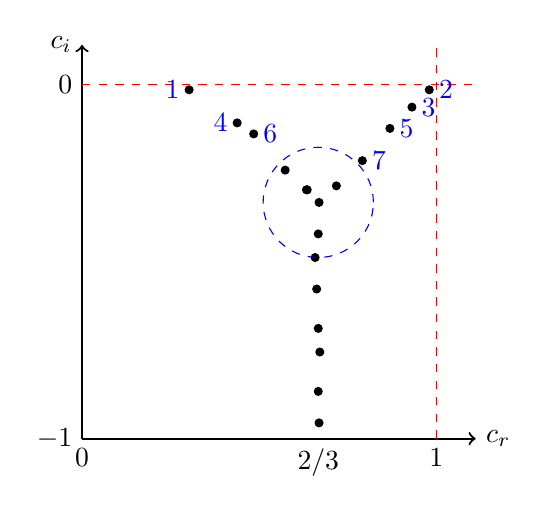
\begin{tikzpicture}
		\draw[thick,->] (0,0) -- (5, 0) node[right] {$c_r$};
		\draw[thick,->] (0,0) -- (0, 5) node[left] {$c_i$};
		\draw (0,0) node[below] {$0$};
		\draw (4.5,0) node[below] {$1$};
		\draw (0,0) node[left] {$-1$};
		\draw (0,4.5) node[left] {$0$};
		\draw (3, 0) node[below] {$2/3$};
		\draw[red,dashed] (4.5, 0) -- (4.5, 5);
		\draw[red,dashed] (0, 4.5) -- (5, 4.5);
		\draw[fill] (3.01, 0.2) circle (0.05);
		\draw[fill] (3, 0.6) circle (0.05);
		\draw[fill] (3.02, 1.1) circle (0.05);
		\draw[fill] (3, 1.4) circle (0.05);
		\draw[fill] (2.98, 1.9) circle (0.05);
		\draw[fill] (2.96, 2.3) circle (0.05);
		\draw[fill] (3, 2.6) circle (0.05);
		\draw[fill] (3.01, 3) circle (0.05);
		\draw[fill] (3.23, 3.21) circle (0.05);
		\draw[fill] (3.56, 3.53) circle (0.05);
		\draw[fill] (3.91, 3.94) circle (0.05);
		\draw[fill] (4.19, 4.21) circle (0.05);
		\draw[fill] (4.41, 4.43) circle (0.05);
		\draw[fill] (2.85, 3.16) circle (0.05);
		\draw[fill] (2.58, 3.41) circle (0.05);
		\draw[fill] (1.97, 4.01) circle (0.05);
		\draw[fill] (1.36, 4.43) circle (0.05);
		\draw[fill] (2.18, 3.87) circle (0.05);
		\draw[fill] (2.86, 3.16) circle (0.05);
		\draw[blue] (4.41, 4.43) node[right] {$2$};
		\draw[blue] (1.36, 4.43) node[left] {$1$};
		\draw[blue] (4.19, 4.21) node[right] {$3$};
		\draw[blue] (1.97, 4.01) node[left] {$4$};
		\draw[blue] (3.91, 3.94) node[right] {$5$};
		\draw[blue] (2.18, 3.87) node[right] {$6$};
		\draw[blue] (3.56, 3.53) node[right] {$7$};
		\draw[blue,dashed] (3,3) circle (0.7);
	\end{tikzpicture}
\end{center}

Once again, note that eigenvalue with imaginary part close to $0$. At $\ReN =
5772$, this eigenvalue becomes unstable. Numbering the eigenvalues by
descending imaginary part, we can ask how many eigenvalues are required for an
accurate estimate of $G$? It turns out we just need to include the `neck' of
the $Y$-shape, circled in blue. This corresponds to the first 15 (roughly)
eigenvalues.

\begin{center}
	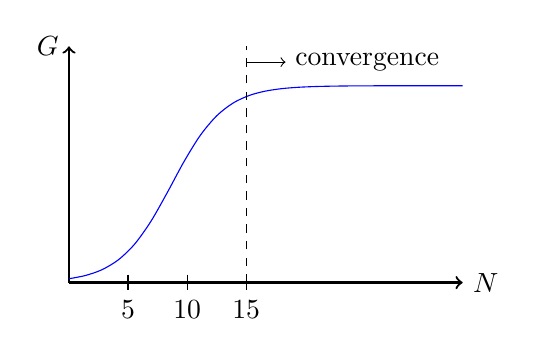
\begin{tikzpicture}
		\draw[thick,->] (0,0) -- (5, 0) node[right] {$N$};
		\draw[thick,->] (0,0) -- (0, 3) node[left] {$G$};
		\draw[blue,smooth] plot[domain=0:5] ({\x},{1/(0.4+exp(-3*(\x-1)))});
		\draw (0.75, 0.1) -- (0.75, -0.1) node[below] {$5$};
		\draw (1.5, 0.1) -- (1.5, -0.1) node[below] {$10$};
		\draw (2.25, 0.1) -- (2.25, -0.1) node[below] {$15$};
		\draw[dashed] (2.25, 0) -- (2.25, 3);
		\draw[->] (2.25, 2.8) -- (2.75, 2.8);
		\draw (2.75, 2.8) node[right] {convergence};
	\end{tikzpicture}
\end{center}

A plot of max growth rate $G$ against time $T$ demonstrates an \emph{envelope} --
there is not necessarily a mode which matches the maximum growth rate at all
times $T$, but instead numerous different modes which may yield the maximum
growth rate at a \emph{specific} time $T$. The envelope decays for large $T$
as only linear instability modes remain. The key point is that the optimal
initial conditions depend on the time $T$ at which $G$ should be maximised.

\begin{center}
	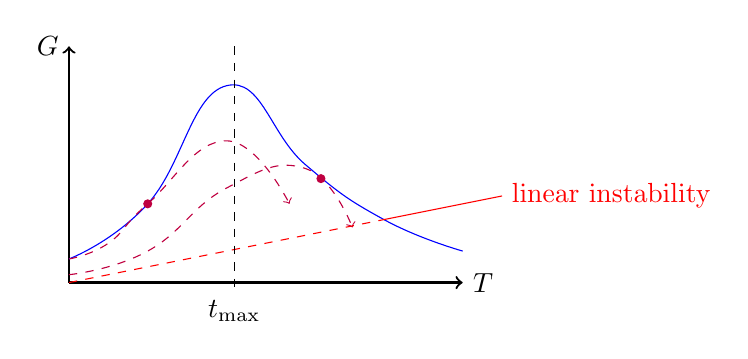
\begin{tikzpicture}
		\draw[thick,->] (0,0) -- (5, 0) node[right] {$T$};
		\draw[thick,->] (0,0) -- (0, 3) node[left] {$G$};
		\draw[blue,smooth] plot[tension=0.8] coordinates {(0, 0.3) (1, 1) (2, 2.5)
			(3, 1.5) (4, 0.8) (5, 0.4)};
		\draw[purple,dashed,->,smooth] plot[tension=0.8] coordinates {(0, 0.3)
			(0.5, 0.5) (1, 1) (2, 1.8) (2.8, 1)};
		\draw[purple,fill] (1, 1) circle (0.05);
		\draw[purple,dashed,->,smooth] plot[tension=0.8] coordinates {(0, 0.1)
		(1, 0.4) (2, 1.2) (3, 1.45) (3.6, 0.7)};
		\draw[purple,fill] (3.2, 1.32) circle (0.05);
		\draw[red,dashed] (0,0) -- (4, 0.8);
		\draw[red] (4, 0.8) -- (5.5, 1.1) node[right] {linear instability};
		\draw[dashed] (2.1, 3) -- (2.1, -0.1) node[below] {$t_{\max}$};
	\end{tikzpicture}
\end{center}

\paragraph{Optimal growth in wall-bounded shear flows.}
The optimal growth gains $G$ and the time $t_{\max}$ at which this maximum is
reached is shown in the table below for a some canonical wall-bounded shear
flows. 
\begin{table}
	\centering
	\begin{tabular}{c|ccccc}
		& $G$ & $t_{\max}$ & $\alpha$ & $\beta$ & ref.\\ \hline
		PPF & $2\times 10^{-4} \ReN^2$ & $0.076\ReN$ & 0 & 2.04 & (1) \\
		PCF & $1.2\times 10^{-3} \ReN^2$ & $0.117\ReN$ & $\frac{35}{\ReN}$ &
		1.6 & (1) \\
		Pipe flow & $7\times 10^{-5} \ReN^2$ & $0.048\ReN$ & 0 & 1 & (2) \\
		Blasius BL & $1.5\times 10^{-3} \ReN^2$ & $0.778\ReN$ & 0 & 0.65 & (3) \\
	\end{tabular}
\end{table}

Notice in particular that the maximum growth gain $G \sim \ReN^2$ and
$t_{\max} \sim \ReN$. Also, the maximum growth has $\beta$ non-zero (2D
spanwise variation) in contrast to Squire's theorem (2D streamwise variation).
References:
\begin{enumerate}
	\item Trefethen et al. (1993)
	\item Schmid \& Henningson (1994)
	\item Butler \& Farrel (1992)
\end{enumerate}

\subsection{Mechanisms of transient growth}
Take the $(v, \eta)$ equations 
\begin{align}
	\left(\frac{\partial}{\partial t} + U \frac{\partial}{\partial x}\right)
	\eta + \frac{\partial v}{\partial z} \frac{\diffd U}{\diffd y} &=
	\frac{1}{\ReN} \nabla^2 \eta \\
	\left(\frac{\partial}{\partial t} + U \frac{\partial}{\partial x}\right)
	\nabla^2 v - \frac{\partial v}{\partial x} \frac{\diffd^2 U}{\diffd y^2}
								&= \frac{1}{\ReN} \nabla^4 v
\end{align}
and consider infinite shear $U(y) = \alpha y$ in an unbounded domain.
\begin{center}
	\begin{tikzpicture}
		\draw[thick,->] (-2, 0) -- (2, 0) node[right] {$x$};
		\draw[thick,->] (0, -2) -- (0, 2) node[left] {$y$};
		\draw[thick,blue] (1,2) -- (-1, -2);
		\draw[blue,->] (0, 0.5) -- (0.25, 0.5);
		\draw[blue,->] (0, 1) -- (0.5, 1);
		\draw[blue,->] (0, 1.5) -- (0.75, 1.5);
		\draw[blue,->] (0, -0.5) -- (-0.25, -0.5);
		\draw[blue,->] (0, -1) -- (-0.5, -1);
		\draw[blue,->] (0, -1.5) -- (-0.75, -1.5);
	\end{tikzpicture}
\end{center}

Note $\left[\alpha\right] = T^{-1}, \left[\nu\right] = L^2 T^{-1}$ are the
only parameters in the problem so we
cannot define an inherent lengthscale which is independent of $\ReN$ (i.e. if
we used $\nu, \alpha$ to form a lengthscale, $\ReN \sim 1$ necessarily.)
Hence we return to units:
\begin{align}
	\left(\frac{\partial}{\partial t} + \alpha y \frac{\partial}{\partial x}\right)
	\nabla^2 v -\nu \nabla^4 v &= 0 \label{eq:l12:1}\\
	\left(\frac{\partial}{\partial t} + \alpha y \frac{\partial}{\partial x}\right)
	\eta - \nu \nabla^2 \eta &= -\alpha \frac{\partial v}{\partial z}
	\label{eq:l12:2}
\end{align}

Recall $\eta \equiv \hat{\symbf{y}}\cdot\nabla \times \u = u_z - w_x$. Look
for \emph{Kelvin modes} of the form
\begin{equation}
	\left[v,\eta\right](\x,t) =
	\left[\hat{v},\hat{\eta}\right](t)e^{i\symbf{k}(t)\cdot\x}
\end{equation}

From \eqref{eq:l12:1} we have
\begin{align}
	\left(\frac{\partial}{\partial t} + \alpha y \frac{\partial}{\partial
	x}\right) \left(-\k^2(t)\hat{v}(t)e^{i\k(t)\cdot\x}\right) 
	&= \nu \k^4 \hat{v}e^{i\k\cdot\x} \\
	-(\k^2 \hat{v})_t e^{i\k\cdot\x} - \k^2
	\hat{v}(i\k_t\cdot\x)e^{i\k\cdot\x} - \alpha \k^2 y
	\hat{v}(ik_1)e^{i\k\cdot\x} &= \nu \k^4 \hat{v}e^{i\k\cdot\x} \\
	-(\k^2\hat{v})_t - i\k_t\cdot\x\k^2\hat{v} - \alpha \k^2 y \hat{v}ik_1
								&= \nu \k^4 \hat{v}
\end{align}
Separating into components which are $\x$-dependent and $\x$-independent gives
\begin{align}
	-(\k^2\hat{v})_t &= \nu \k^4 \hat{v} \label{eq:l12:3}\\
	-i\k_t\cdot\x - \alpha k_1 y &= 0 \label{eq:l12:4}
\end{align}
The second equation \eqref{eq:l12:4} can also be written
\begin{equation}
	\dot{k}_1 x + \dot{k}_2 y + \dot{k}_3 z + \alpha k_1 y = 0
\end{equation}
Hence $\dot{k}_1 = \dot{k}_3 = 0$ and $\dot{k}_2 = -\alpha k_1$ so
\begin{align}
	k_1 &= k_{01} \\
	k_2 &= k_{02} - \alpha k_{01} t \\
	k_3 &= k_{03}
\end{align}
Now \eqref{eq:l12:3} can be written
\begin{align}
	(\k^2 \hat{v})_t &= -\nu \k^2 (\k^2 \hat{v}) \\
	\implies \k^2 \hat{v} &= \k_0^2 \hat{v}(0) e^{-\nu \int_0^t
	\k^2(\tau)\,\diffd \tau} \\
		\implies \hat{v}(t) &= \frac{\k_0^2}{\k^2(t)} \hat{v}(0) e^{-\nu \int_0^t
	\k^2(\tau)\,\diffd \tau} 
\end{align}

Then from \eqref{eq:l12:2}
\begin{equation}
	\hat{\eta}_t + \nu \k^2(t)\hat{\eta} = -i\alpha k_3 \hat{v}(t)
\end{equation}
It is useful to look at two 2D special cases.
\paragraph{2D with $\partial_z = 0$ (no spanwise variation).}
If there is no spanwise variation then $k_3 = 0$ and all the `action' is in
the $\hat{v}$ equation, as the $\hat{\eta}$ equation is unforced. We have
\begin{equation}
	\hat{v}(t) = \hat{v}(0)\frac{k_{01}^2 + k_{02}^2}{k_{01}^2 +
	(k_{02}-\alpha k_{01}t)^2}e^{-\nu \int_0^t
	\k^2(\tau)\,\diffd \tau} 
\end{equation}
If $k_{02} \gg k_{01}$, we expect large growth on `fast' times
$\mathcal{O}(1)$, as opposed to $\mathcal{O}(1/\nu)$ times. We see this as
follows: denote the $\k_0^2/\k^2$ factor as $A$. Then
\begin{itemize}
	\item At $t=0$, $A \sim 1$.
	\item At $t=k_{02}/\alpha k_{01}$, $A \to \frac{k_{02}^2}{k_{01}^2} \gg
		1$.
	\item At $t=2k_{02}/\alpha k_{01}$, $A \to 1$.
\end{itemize}
Incompressibility combined with $\u = \hat{u}(t)\exp(i\k(t)\cdot\x)$ gives
\begin{equation}
	ik_1 \hat{u} = i k_2 \hat{v} = 0
\end{equation}
i.e. $\k$ is perpendicular to $(u,v)$.

\begin{center}
	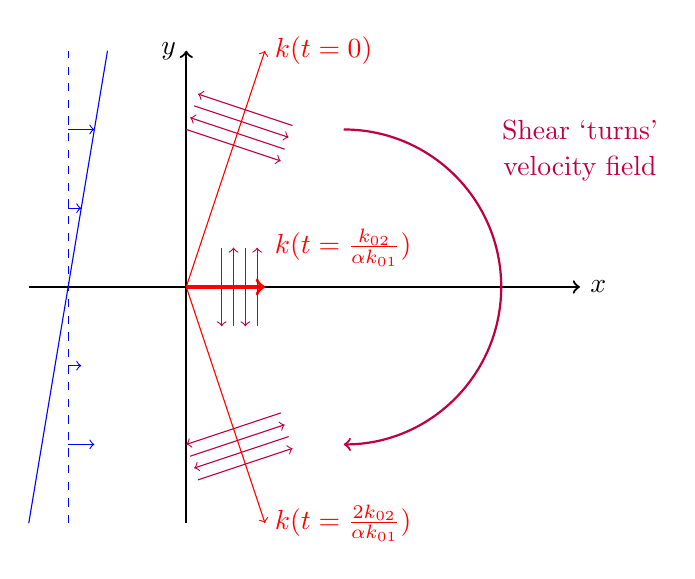
\begin{tikzpicture}
		\draw[thick,->] (-2,0) -- (5,0) node[right] {$x$};
		\draw[thick,->] (0, -3) -- (0, 3) node[left] {$y$};
		\draw[blue,dashed] (-1.5, -3) -- (-1.5, 3);
		\draw[blue] (-1, 3) -- (-2, -3);
		\draw[blue,->] (-1.5,1) -- (-1.5+0.33333/2,1);
		\draw[blue,->] (-1.5,2) -- (-1.5+0.33333,2);
		\draw[blue,->] (-1.5,-1) -- (-1.5+0.33333/2,-1);
		\draw[blue,->] (-1.5,-2) -- (-1.5+0.33333,-2);
		\draw[red,->] (0,0) -- (1, 3) node[right] {$\k(t=0)$};
		\draw[red,->] (0,0) -- (1, -3) node[right] {$\k(t=\frac{2k_{02}}{\alpha
		k_{01}})$};
		\draw[very thick,red,->] (0,0) -- (1,0);
		\draw[red] (1, 0.5) node[right] {$\k(t=\frac{k_{02}}{\alpha k_{01}})$};
		\draw[purple,->] (0,2) -- (1.2, 1.6);
		\draw[purple,<-] (0.05,2.15) -- (1.25, 1.75);
		\draw[purple,->] (0.1,2.3) -- (1.3, 1.9);
		\draw[purple,<-] (0.15,2.45) -- (1.35, 2.05);
		\draw[purple,<-] (0.9, 0.5) -- (0.9, -0.5);
		\draw[purple,->] (0.75, 0.5) -- (0.75, -0.5);
		\draw[purple,<-] (0.6, 0.5) -- (0.6, -0.5);
		\draw[purple,->] (0.45, 0.5) -- (0.45, -0.5);
		\draw[purple,<-] (0,-2) -- (1.2,- 1.6);
		\draw[purple,->] (0.05,-2.15) -- (1.25,- 1.75);
		\draw[purple,<-] (0.1,-2.3) -- (1.3,- 1.9);
		\draw[purple,->] (0.15,-2.45) -- (1.35,- 2.05);
		\draw[purple,thick,->] (2, 2) arc (90:-90:2);
		\draw[purple] (5, 2) node {Shear `turns'};
		\draw[purple] (5, 1.5) node {velocity field};
	\end{tikzpicture}
\end{center}

This is the \emph{Orr mechanism} (1907). The energy is maximised at $t=
k_{02}/\alpha k_{01}$. The initial conditions point into the shear, with the
energy growth arising as the shear `rotates' the velocity field. It is a 2D
mechanism, inviscid (happens quickly), and growth is $\mathcal{O}(\ReN^0)$.

\paragraph{2D with $\partial_x = 0$ (no streamwise variation).}
If there is no streamwise variation then $k_1 = 0$, hence $k$ is constant.
Then
\begin{align}
	\hat{v}(t) &= \hat{v}(0) e^{-\nu \k^2 t} \\
	\hat{\eta} + \nu \k^2 \hat{\eta} &= -i\alpha k_3 \hat{v} = -i\alpha k_3
	\hat{v}(0) e^{-\nu \k^2 t} \\
	\implies \left(\hat{\eta}e^{\nu \k^2 t}\right)_t &= -i\alpha k_3
	\hat{v}(0) \\
	\implies \hat{\eta}(t) &= \hat{\eta}_0 e^{-\nu \k^2 t} - i\alpha k_3 t
	\hat{v}(0) e^{-\nu \k^2 t}
\end{align}

The exponential factors damp $\hat{\eta}$, but the $t$ factor in the second
term provides the possibility of algebraic growth. In the case of no
streamwise variation we have $\eta = i k_3 u$, so
\begin{equation}
	\hat{u}(t) = \left[ \hat{u}(0) - \alpha t \hat{v}(0)\right] e^{-\nu \k^2
	t}
\end{equation}
Hence we expect algebraic growth in $\hat{u}$ of amplitude
$\mathcal{O}(1/\nu)$, so growth in energy of order $\mathcal{O}(1/\nu^2) =
\mathcal{O}(\ReN^2)$. This explains the previous observations that $G_{\max}
= \mathcal{O}(\ReN^2)$ and $t_{\max} = \mathcal{O}(\ReN)$. This is the
\emph{lift-up mechanism} whereby small, slowly decaying velocities advect
fluid across the shear.

\begin{center}
	\begin{tikzpicture}
		\draw (0,0) -- (5,0) -- (6, 1.5) -- (1, 1.5) -- (0,0);
		\draw[blue,dashed] (2.5, 0.5) -- (2.5, 3);
		\draw[blue, smooth] plot[tension=0.8] coordinates {(2.5, 0.5) (3.4,
		1.5) (3.6, 3)};
		\draw[blue,->] (2.5, 1.6) -- (3.42, 1.6);
		\draw[blue,->] (2.5, 2.5) -- (3.58, 2.5);
		\draw[blue] (3.65, 2.5) node[right] {basic shear};
		\draw[purple] (4.5, 0.8) ellipse (0.15 and 0.3);
		\draw[purple] (1.5, 0.8) [partial ellipse = 90:270:0.15 and 0.3];
		\draw[purple] (4.5, 1.1) -- (1.5, 1.1);
		\draw[purple] (4.5, 0.5) -- (1.5, 0.5);
		\draw[purple,->,thick] (4, 0.8) [partial ellipse = 70:240:0.2 and
		0.4];
		\draw[purple,->,thick] (3, 0.8) [partial ellipse = 70:240:0.2 and
		0.4];
		\draw[purple,->,thick] (2, 0.8) [partial ellipse = 70:240:0.2 and
		0.4];
		\draw[purple] (6, 0.8) node[right] {streamwise rolls};
	\end{tikzpicture}
\end{center}

Streamwise rolls advect slower flowing fluid away from the boundary and faster
flowing fluid towards the boundary. This causes a large anomaly in the
streamwise flow component. Streamwise rolls decay over a $\mathcal{O}(\ReN)$
timescale, which gives $\mathcal{O}(\ReN^2)$ growth.

\subsection{Orr-Sommerfeld operator is non-normal}
The adjoint operator is dependent on the choice of the inner product. Recall
$D \equiv \diffd/\diffd y$ and define the inner product here as
\begin{align}
	\langle \v_1, \v_2 \rangle &\equiv \int_{-1}^1 (D\v_1)^*(D\v_2) + k^2
	\v_1^*\v_2 \, \diffd y \\
							   &= \int_{-1}^1 \v_1^*\left[(k^2-D^2)\v_2\right]
							   \, \diffd y
\end{align}
Hence we have
\begin{align}
	\langle \v_1, \L_{os}\v_2\rangle &= \int_{-1}^1 \v_1^*(k^2-D^2)\{
		\frac{1}{D^2 -k^2} \left[ \frac{1}{\ReN} (D^2 -k^2)^2 - i\alpha
	U(D^2-k^2) + i\alpha D^2 U\right]\}\v_2 \,\diffd y \\
									 &= \langle \L_{os}^\dagger \v_1, \v_2
									 \rangle
\end{align}
by definition of $\L_{os}^\dagger$. Hence the adjoint may be written
\begin{equation}
	\L_{os}^\dagger = 	\frac{1}{D^2 -k^2} \left[i\alpha
	U(D^2-k^2) + 2i\alpha DUD+ \frac{1}{\ReN} (D^2 -k^2)^2 \right]
\end{equation}
It can be shown that $\langle \v_1, \L_{os}^\dagger \L_{os} \v_2 \rangle \ne
\langle \v_1, \L_{os}\L_{os}^\dagger \v_2 \rangle$ for all $\v_1, \v_2$. Hence
$\L_{os}$ is a non-normal operator, so we can expect energy growth even if the
eigenvalues of $\L_{os}$ indicate damping.

\subsection{Energy stability analysis}
Consider the Navier-Stokes equations with a specified velocity boundary condition
$\u = \U_b$ on $\partial V$. Suppose there is a steady basic flow $\U(\x)$.
Consider disturbances to the basic state $\u = \U + \hat{\u}, p = P +
\hat{p}$. The Navier-Stokes equations become
\begin{align}
	\nabla \cdot \hat{\u} &= 0 \\
	\frac{\partial \hat{\u}}{\partial t} + \U \cdot \nabla \hat{\u} +
	\hat{\u}\cdot\nabla \U + \nabla \hat{p} - \frac{1}{\ReN} \nabla^2 \hat{\u}
						  &= - \hat{\u}\cdot\nabla \hat{\u} \label{eq:l13:1}\\
		\implies \frac{\partial \hat{\u}}{\partial t} - \L
	\hat{\u} &= -\hat{\u}\cdot\nabla \hat{\u} \label{eq:l13:2}
\end{align}
where $\L$ is defined by \eqref{eq:l13:1}. The boundary conditions on
$\hat{\u}$ are $\hat{\u} = 0$ on $\partial V$. Using energy norm $\langle \u,
\v \rangle = \int \u \cdot \v \, \diffd V$, apply to disturbance equation
\eqref{eq:l13:2} by taking $\langle \hat{\u},\eqref{eq:l13:2}\rangle$ to get
\begin{equation}
	\frac{\partial}{\partial t} \langle \frac{1}{2}\hat{\u}^2\rangle  =
	\langle \hat{\u}, \L\hat{\u}\rangle - \langle \hat{\u},
	\hat{\u}\cdot\nabla\hat{\u} \rangle
\end{equation}
The last term vanishes since
\begin{align}
	\int \hat{\u} \cdot (\hat{\u}\cdot\nabla\hat{\u}) \, \diffd V 
	&= \int \hat{\u}\cdot\nabla(\frac{1}{2}\hat{\u}^2) \, \diffd V \\
	&= \int \nabla \cdot (\frac{1}{2}\hat{\u}^2 \hat{\u}) -
\cancel{\frac{1}{2}\hat{\u}^2 \nabla \cdot \hat{\u}} \, \diffd V \\
	&= \oint_{\partial V} \frac{1}{2} \hat{\u}^2 \hat{\u}\cdot\diffd \symbf{S}
	= 0
\end{align}
		
We now split the operator $\L$ into symmetric and anti-symmetric parts:
\begin{equation}
\frac{\partial}{\partial t} \langle \frac{1}{2}\hat{\u}^2 \rangle = \langle
\hat{\u}, \frac{1}{2}(\L + \L^\dagger)\hat{\u}\rangle + \langle \hat{\u},
\frac{1}{2}(\L-\L^\dagger)\hat{\u}\rangle
\end{equation}
Once again the last term vanishes since
\begin{equation}
	\langle \hat{\u}, \frac{1}{2}(\L-\L^\dagger)\hat{\u}\rangle = \frac{1}{2}
	\langle \hat{\u}, \L \hat{\u} \rangle - \frac{1}{2}\langle \L \hat{\u},
	\hat{\u} \rangle = 0
\end{equation}
by definition of the adjoint $\L^\dagger$ and symmetry of the inner product.
Thus we have
\begin{equation}
	\frac{\partial}{\partial t} \langle \frac{1}{2}\hat{\u}^2 \rangle = \langle
	\hat{\u}, \frac{1}{2}(\L + \L^\dagger)\hat{\u}\rangle
\end{equation}
Note that $\L + \L^\dagger$ is a self-adjoint operator:
$(\L+\L^\dagger)^\dagger = \L^\dagger + \L$. Hence it is normal with real
eigenvalues. For energy growth (LHS $> 0$) we need an eigenvalue of $\L +
\L^\dagger$ to be positive. Recall, for linear instability, we need an
eigenvalue of $\L$ to have a positive real part.

Let $\ReN_E$ be the first Reynold's number for energy growth and
$\ReN_L$ be the linear instability threshold. Then generically
\begin{equation}
	0 \le \ReN_E \le \ReN_L
\end{equation}
The first inequality is usually strict (Serrin, 1959) and the region $\ReN_E
\le \ReN \le \ReN_L$ is the region where energy growth is possible without
eigenvalue instability. 

\begin{eg}
	For Plane Couette Flow (PCF), $\ReN_E = 20.67$ and $\ReN_L = \infty$. For
	$0 \le \ReN < \ReN_E$ no growth is possible at all, hence the basic flow
	$\U$ is a global attractor: all initial conditions will decay back to the
	basic flow.
\end{eg}

\begin{eg}
	For a uniformly rotating flow, in the rotating frame the Navier-Stokes
	equations are
	\begin{equation}
		\frac{\partial \u}{\partial t} + 2\symbf{\Omega} \times \u + \u \cdot
		\nabla \u + \nabla p = \frac{1}{\ReN} \nabla^2 \u
	\end{equation}
	as well as $\nabla \cdot \u = 0$ and we use boundary condition $\u =
	\symbf{0}$ on $\partial V$ which is the boundary of some region under
	consideration (e.g. for an object in the uniformly rotating flow,
	$\partial V$ is the objects surface). Energy stability analysis gives
	\begin{equation}
		\frac{\partial}{\partial t} \langle \frac{1}{2}\u^2\rangle =
		-\frac{1}{\ReN} \langle \abs{\nabla \u}^2\rangle < 0
	\end{equation}
	so the flow is absolutely stable.
\end{eg}

\subsection{Time stepping to growth}
The matrix/SVD approach to calculating transient growth is only really
feasible for 1D or possibly 2D problems because of the size of the matrices. A
better approach is a matrix-free method which is extendable to time-dependent
problems, different norms, and \emph{adding non-linearity}.

\subsubsection{Constrained optimisation (linear)}
Consider the energy growth of small disturbances on top of a base flow
$\u_{\text{lam}}$ by forming the Lagrangian
\begin{align}
	G &= G(\u, p, \lambda, \symbf{\nu}, \pi; T) \\
	  &= \langle \frac{1}{2} \abs{\u(\x, T)}^2\rangle &&\text{objective
	  functional}\\
	  &+ \lambda(\x,t) \left[ \langle \frac{1}{2}\abs{\u(\x,0)}^2\rangle -1 \right]
	  &&\text{initial amplitude condition} \\
	  &+ \int_0^T \langle \symbf{\nu}(\x,t) \cdot \left[ \frac{\partial
	  \u}{\partial t} + \u_{\text{lam}} \cdot \nabla \u + \u \cdot \nabla
	  \u_{\text{lam}} + \nabla p - \frac{1}{\ReN} \nabla^2 \u \right] \rangle
	\, \diffd t &&\text{satisfies NS equations} \\
				&+ \int_0^T \langle \pi(\x,t) \nabla \cdot \u \rangle \,
	\diffd t &&\text{satisfies incompressibility}
\end{align}
where $\langle \chi \rangle \equiv \int \chi \, \diffd V$. The first term is
the energy functional to be optimisied, and the remaining terms enforce unit
initial amplitude, Navier-Stokes, and incompressibility via Lagrange
multipliers $\lambda, \symbf{\nu}, \pi$ respectively. The Euler-Lagrange
equations to `stationarise' $G$ follow by expanding perturbations $\u
+\delta\u, p + \delta p$, etc. and requiring the \emph{first variations}
$\frac{\delta G}{\delta \u}, \frac{\delta G}{\delta p}$, etc. vanish. For
variations of $p$ we have
\begin{align}
	0 = \int_0^T \langle \frac{\delta G}{\delta p} \delta p \rangle \, \diffd
	t  &\equiv \int_0^T \langle \symbf{\nu}\cdot\nabla \delta p\rangle \,
	\diffd t \\
	   &= \int_0^T \langle \nabla \cdot (\symbf{\nu} p) - \delta p \nabla
	   \cdot \symbf{\nu} \rangle \, \diffd t \\
	   &= \int_0^T \oint \symbf{\nu} \delta p \cdot \diffd \symbf{S} - \langle
	   \delta p \nabla \cdot \symbf{\nu} \rangle \, \diffd t
\end{align}
Hence we require $\symbf{\nu} = \symbf{0}$ on $\partial V$ and $\nabla \cdot
\symbf{\nu} = 0$ throughout $V$. Now consider variations of $\u$ (with
$\delta \u = \symbf{0}$ on $\partial V$)
\begin{align}
	0 = \int_0^T \langle \frac{\delta G}{\delta \u} \cdot \delta \u\rangle \,
	\diffd t &= \langle \u(\x, T) \delta \u(\x, T)\rangle + \lambda \langle
	\u(\x, 0) \cdot \delta \u(\x, 0)\rangle + \int_0^T \langle \pi \nabla
	\cdot \delta \u\rangle \, \diffd t \\
			 &+ \int_0^T \langle \symbf{\nu}\cdot\left[\frac{\partial \delta
			 \u}{\partial t} + \u_{\text{lam}} \cdot \nabla \delta \u + \delta
			 \u \cdot \nabla \u_{\text{lam}} - \frac{1}{\ReN} \nabla^2 \delta
			 \u \right] \rangle \, \diffd t \\
			 &= \langle \delta \u(\x,T) \cdot\left[ \u(\x, T) +
			 \symbf{\nu}(\x, T) \right] \rangle + \langle \delta \u(\x,0)
			 \cdot \left[ \lambda \u(\x, 0) - \symbf{\nu}(\x, 0)\right]
			 \rangle \\
			 &+ \int_0^T \langle \delta \u \cdot \left[ -\frac{\partial
			 \symbf{\nu}}{\partial t} - \u_{\text{lam}} \cdot \nabla
			 \symbf{\nu} + \symbf{\nu} \cdot (\nabla \u_{\text{lam}})^T -
			 \nabla \pi - \frac{1}{\ReN} \nabla^2 \symbf{\nu} \right] \rangle
			 \, \diffd t
\end{align}

The expression $\left[\dots\right]$ in the final integral is called the
\emph{dual (linearised) Navier-Stokes equation}. Hence for $\frac{\delta
G}{\delta \u} = 0$ we have
\begin{align}
	\u(\x, T) + \symbf{\nu}(\x, T) &= 0 \label{eq:l13:3} \\
	\lambda \u(\x, 0) - \symbf{\nu}(\x, 0) &= 0 \label{eq:l13:4}\\
	\frac{\partial \symbf{\nu}}{\partial t} + \u_{\text{lam}} \cdot \nabla
	\symbf{\nu} - \symbf{\nu} \cdot (\nabla \u_{\text{lam}})^T + \nabla \pi +
	\frac{1}{\ReN} \nabla^2 \symbf{\nu} &= 0 \hspace{1em}\forall t \in
	\left[0,T\right] \label{eq:l13:5}
\end{align}
These together with equations imposed by the Lagrange multipliers must all be
solved. The system of equations are solved iteratively as follows.
\begin{enumerate}
	\item Choose $\u^{(0)}(\x, 0)$ such that 
		\begin{equation}
			\langle \frac{1}{2}\abs{\u^{(0)}(\x, 0)}^2\rangle = 1
		\end{equation}
		Then construct $\u^{(n+1)}(\x,0)$ from $\u^{(n)}(\x,0)$ as follows.
	\item Solve the linearised Navier-Stokes equations to time step from $t=0$
		to $t=T$ to get $\u^{(n)}(\x,0)$.
	\item Use constraint \eqref{eq:l13:3} to find $\symbf{\nu}^{(n)}(\x,T) =
		-\u^{(n)}(\x, T)$.
	\item Solve the lineariseed dual Navier-Stokes equations to time step
		backwards from $t=T$ to $t=0$ to get $\symbf{\nu}^{(n)}(\x,0)$. Note
		time-stepping backwards is natural as $\symbf{\nu}$ satisfies an
		`anti-diffusion' equation of the form $\symbf{\nu}_t \sim -\nabla^2
		\symbf{\nu}$.
	\item Use the result (prior to imposing \eqref{eq:l13:4})
		\begin{equation}
			\frac{\partial G}{\partial \delta \u(\x,0)} = \lambda
			\u^{(n)}(\x,0) - \symbf{\nu}(\x, 0)
		\end{equation}
		to step $\u$ to increase $G$. This may be achieved via \emph{steepest
		ascent}:
		\begin{equation}
			\u^{(n+1)}(\x,0) = \u^{(n)}(\x,0) + \veps \left[ \frac{\delta
			G}{\delta \u^{(n)}(\x,0)}\right]
		\end{equation}
		i.e. take a small step $\veps$ in the direction where $G$ increases.
		Then
		\begin{equation}
			\u^{(n+1)}(\x,0) = \u^{(n)}(\x,0) + \veps(\lambda \u^{(n)}(\x,0) -
			\symbf{\nu}^{(n)}(\x,0))
		\end{equation}
		with $\lambda$ chosen such that 
		\begin{equation}
			 1 = \frac{1}{2}\langle \abs{\u^{(n+1)}(\x,0)}^2\rangle
		 \end{equation}
		 Here, $\veps$ is a small adjustable stepping parameter.
\end{enumerate}

\begin{center}
	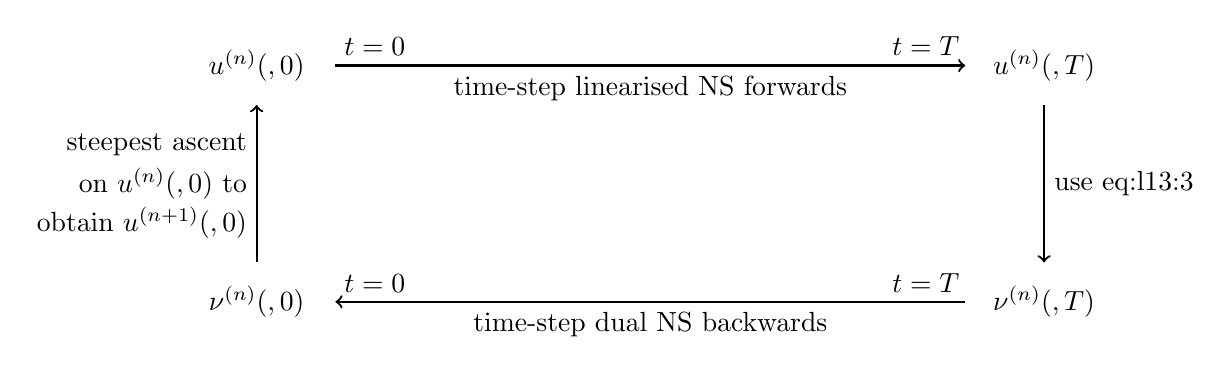
\begin{tikzpicture}
		\draw (0,0) node {$\u^{(n)}(\x,0)$};
		\draw[thick,->] (1, 0) -- (9, 0) node[midway,below] {time-step
		linearised NS forwards};
		\draw (1.5, 0) node[above] {$t=0$};
		\draw (8.5, 0) node[above] {$t=T$};
		\draw (10, 0) node {$\u^{(n)}(\x,T)$};
		\draw[thick,->] (10, -0.5) -- (10, -2.5) node[midway,right] {use \eqref{eq:l13:3}};
		\draw (10, -3) node {$\symbf{\nu}^{(n)}(\x, T)$};
		\draw[thick,->] (9, -3) -- (1, -3) node[midway, below] {time-step dual
		NS backwards};
		\draw (8.5, -3) node[above] {$t=T$};
		\draw (1.5, -3) node[above] {$t=0$};
		\draw (0, -3) node {$\symbf{\nu}^{(n)}(\x, 0)$};
		\draw[thick,->] (0, -2.5) -- (0, -0.5);
		\draw (0, -1) node[left] {steepest ascent};
		\draw (0, -1.5) node[left] {on $\u^{(n)}(\x,0)$ to};
		\draw (0, -2) node[left] {obtain $\u^{(n+1)}(\x,0)$};
	\end{tikzpicture}
\end{center}

\paragraph{Application.}
Consider flow through a rapid pipe expansion. The flow has a parabolic profile
typical of pipe flow upstream and far downstream of the expansion inlet. Noise
is introduced at the inlet A. Transient growth can mean this noise is
magnified significantly at B but ultimately decays downstream at C if linearly
stable. See Cantwell et al., Phys Fluids, \textbf{22} (2010) 034101.

\begin{center}
	\begin{tikzpicture}
		\draw (0, 0.5) -- (2, 0.5) -- (2, 1.5) -- (7, 1.5);
		\draw (0, -0.5) -- (2, -0.5) -- (2, -1.5) -- (7, -1.5);
		\draw[blue,dashed] (1, 0.5) -- (1, -0.5);
		\draw[blue, smooth] plot[domain=-0.5:0.5] ({1.25-\x*\x},{\x});
		\draw[blue,dashed] (7, 1.5) -- (7, -1.5);
		\draw[blue, smooth] plot[domain=-1.5:1.5] ({7+0.3*1.5*1.5-0.3*\x*\x},{\x});
		\draw[blue,smooth, ->] plot coordinates {(2, 0.5) (2.5, 0.65) (3, 1)};
		\draw[blue,smooth] plot coordinates {(3, 1) (3.5, 1.3) (4, 1.45) (4.5, 1.5)};
		\draw[blue,smooth, ->] plot coordinates {(2, -0.5) (2.5, -0.65) (3, -1)};
		\draw[blue,smooth] plot coordinates {(3, -1) (3.5, -1.3) (4, -1.45) (4.5, -1.5)};
		\draw[blue,rotate=40,->] (2.6, -0.8) [partial ellipse=-90:90:0.45 and 0.25];
		\draw[blue,rotate=40,->] (2.6, -0.8) [partial ellipse=90:270:0.45 and 0.25];
		\draw[blue,rotate=-40,<-] (2.6, 0.8) [partial ellipse=-90:90:0.45 and 0.25];
		\draw[blue,rotate=-40,<-] (2.6, 0.8) [partial ellipse=90:270:0.45 and 0.25];
		\draw[red,smooth] plot[domain=0:1] ({1.3+\x/2},{0.05*sin(deg(25*\x))});
		\draw[red,smooth] plot[domain=0:1.5] ({4+\x/2},{0.5*sin(deg(15*\x))});
		\draw[red,smooth] plot[domain=0:1] ({6+\x/2},{0.01*sin(deg(15*\x))});
		\draw[red] (1.3+0.25,0) node[below] {A};
		\draw[red] (4+0.425,-0.4) node[below] {B};
		\draw[red] (6+0.25,0) node[below] {C};
	\end{tikzpicture}
\end{center}

\paragraph{Comments.}
\begin{itemize}
	\item It is easy to change the objective functional in this method: all
		difficulties lie in handling the governing equation rather than the
		objective functional.
	\item It is easy to handle a basic state $\u_{\text{lam}}(\x,t)$ which is
		time dependent. The matrix approach assumes a steady basic state.
	\item The variational approach can be extended to nonlinear disturbances
		easily.
\end{itemize}

\subsubsection{Constrained optimisation (nonlinear)}
Consider as an example the nonlinear system
\begin{equation}
	\frac{\diffd \x}{\diffd t} = \begin{pmatrix} -x + 10y \\
	y(10e^{-x^1/100}-y)(y-1) \end{pmatrix} = \symbf{f}(\x)
	\label{eq:l14:1}
\end{equation}
See Kerswell et al., Prog. Rep. Phys \textbf{77} (2014) 085901 for a more
in-depth discussion. A phase portrait of this dynamical system may be plotted
with sample trajectories as follows. Red points indicate a fixed point.
\begin{center}
	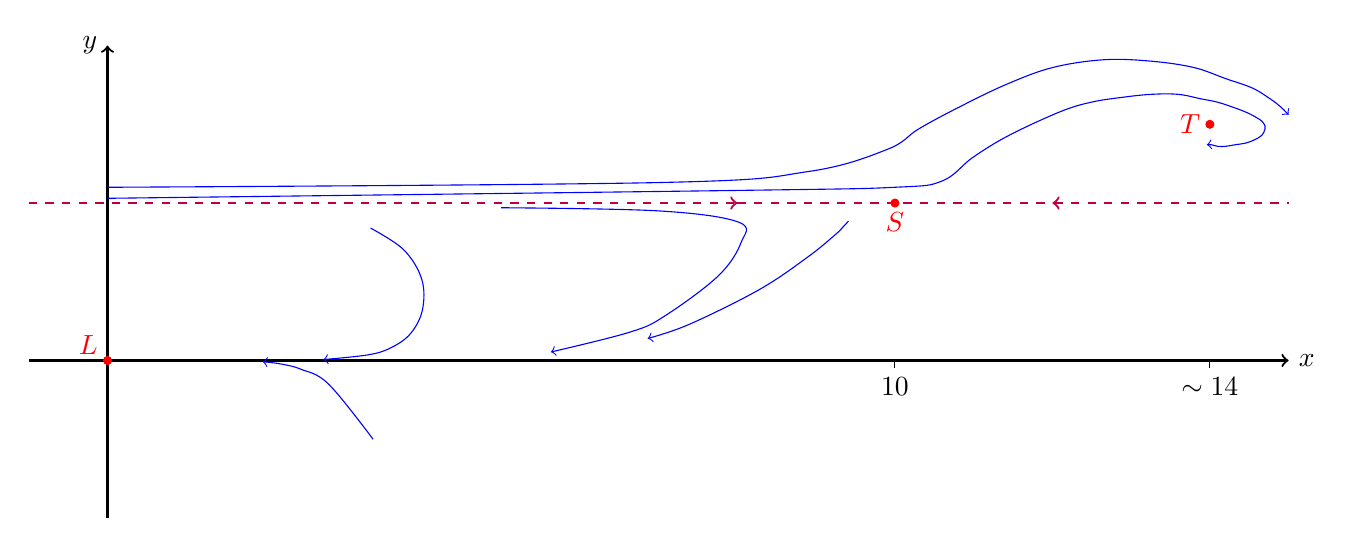
\begin{tikzpicture}
		\draw[thick,->] (-1, 0) -- (15, 0) node[right] {$x$};
		\draw[thick,->] (0, -2) -- (0, 4) node[left] {$y$};
		\draw[dashed, thick, purple,->] (-1, 2) -- (8, 2);
		\draw[dashed, thick, purple] (8, 2) -- (12, 2);
		\draw[dashed, thick, purple,<-] (12, 2) -- (15, 2);
		\draw (10, 0) -- (10, -0.1) node[below] {$10$};
		\draw (14, 0) -- (14, -0.1) node[below] {$\sim14$};
		\draw[red,fill] (0,0) circle (0.05);
		\draw[red] (0,0.2) node[left] {$L$};
		\draw[red,fill] (10,2) circle (0.05);
		\draw[red] (10, 2) node[below] {$S$};
		\draw[red,fill] (14,3) circle (0.05);
		\draw[red] (14, 3) node[left] {$T$};
		\draw[blue,smooth,->] plot[tension=0.6] coordinates {(0, 1.1*2) (7,
			1.13*2) (8.9,
			1.2*2) (9.9, 1.34*2) (10.3, 1.47*2) (10.78,
			1.6*2) (11.4, 1.75*2) (12, 1.86*2) (12.66, 1.91*2) (13.27, 1.9*2)
			(13.8, 1.86*2) (14.2, 1.79*2) (14.54, 1.73*2) (14.77, 1.66*2)
			(14.9, 1.61*2) (15, 1.56*2)};
		\draw[blue,smooth,->] plot[tension=0.6] coordinates {(0, 1.03*2)
			(8, 1.08*2) (10, 1.1*2) (10.6, 1.14*2) (10.99, 1.29*2) (11.45, 1.43*2)
			(12.1, 1.58*2) (12.49, 1.64*2) (12.87, 1.67*2) (13.25, 1.69*2)
			(13.6, 1.69*2) (13.9, 1.66*2) (14.1, 1.64*2) (14.34, 1.6*2)
			(14.49, 1.57*2) (14.6, 1.54*2) (14.66, 1.52*2) (14.7, 1.49*2)
			(14.7, 1.47*2) (14.66, 1.43*2) (14.56, 1.4*2) (14.45, 1.38*2)
			(14.32, 1.37*2) (14.2, 1.36*2) (14.1, 1.36*2) (14.02, 1.37*2)
			(13.96, 1.37*2)};
		\draw[blue,smooth,->] plot[tension=0.6] coordinates {(5, 0.97*2)
			(7, 0.95*2) (8.017, 0.878*2) (8.046, 0.749*2) (7.76, 0.539*2) (7.09, 0.287*2)
			(6.64, 0.181*2) (5.63, 0.054*2)};
		\draw[blue,smooth,->] plot[tension=0.6] coordinates {(9.41,
			0.885*2) (9.34, 0.8475*2) (9.24, 0.798*2) (8.89, 0.656*2)
			(8.28, 0.451*2) (7.39, 0.23*2) (6.86, 0.14*2)};
		\draw[blue,smooth,->] plot[tension=0.6] coordinates {(3.373,
			-0.5*2) (2.808, -0.15*2) (2.454, -0.055*2) (2.19, -0.021*2)
			(1.97, -0.008*2)};
		\draw[blue,smooth,->] plot[tension=0.6] coordinates {(3.34,
			0.841*2) (3.76, 0.704*2) (3.99, 0.517*2) (4, 0.323*2) (3.85,
			0.172*2) (3.6, 0.0812*2) (3.31, 0.036*2) (2.74, 0.006*2)};
	\end{tikzpicture}
\end{center}

The fixed points are labelled $L$ for `laminar' state, $S$ for the saddle on
the basin boundary, and $T$ for `turbulent' state. The basin of attraction of
the fixed point $L$ is $y < 1$. Transient growth appears in a region close to
the origin: consider a `zoomed in' view of the fixed point $L$. The
trajectories temporarily increase distance from the origin, hence there is
brief energy growth.

\begin{center}
	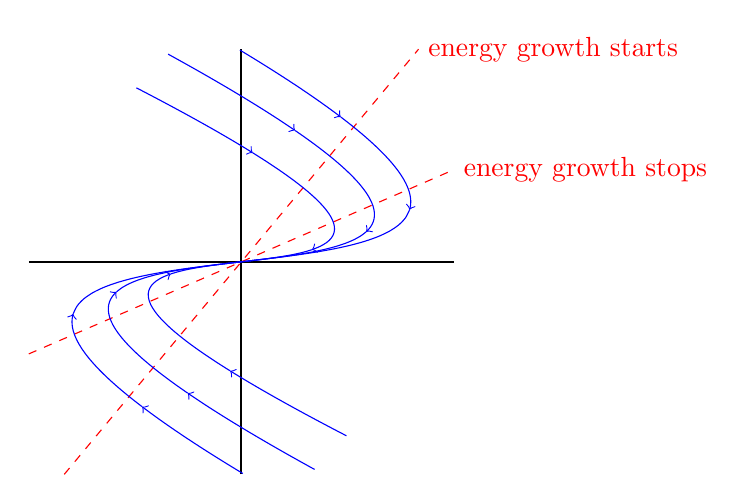
\begin{tikzpicture}[scale=0.9]
		\draw[thick] (-3, 0) -- (3,0);
		\draw[thick] (0, -3) -- (0, 3);
		\draw[red,dashed](-3, -1.3) -- (3, 1.3);
		\draw[red,dashed] (-2.5, -3) -- (2.5, 3);
		\draw[red] (2.5,3) node[right] {energy growth starts};
		\draw[red] (3, 1.3) node[right] {energy growth stops};
		\draw[blue,smooth,rotate=70,->] plot[domain=-1.8:-1.5] ({\x},{\x*\x*\x-2*\x});
		\draw[blue,smooth,rotate=70,->] plot[domain=-2.4:-2]
		({\x},{0.7*0.7*\x*\x*\x-2*\x});
		\draw[blue,smooth,rotate=70,->] plot[domain=-2.8:-2.4]
		({\x},{0.55*0.55*\x*\x*\x-2*\x});
		\draw[blue,smooth,rotate=70,->] plot[domain=-1.5:-0.5] ({\x},{\x*\x*\x-2*\x});
		\draw[blue,smooth,rotate=70,->] plot[domain=-2:-1]
		({\x},{0.7*0.7*\x*\x*\x-2*\x});
		\draw[blue,smooth,rotate=70,->] plot[domain=-2.4:-1.5]
		({\x},{0.55*0.55*\x*\x*\x-2*\x});
		\draw[blue,smooth,rotate=70] plot[domain=-0.5:0.5] ({\x},{\x*\x*\x-2*\x});
		\draw[blue,smooth,rotate=70] plot[domain=-1:1]
		({\x},{0.7*0.7*\x*\x*\x-2*\x});
		\draw[blue,smooth,rotate=70] plot[domain=-1.5:1.5]
		({\x},{0.55*0.55*\x*\x*\x-2*\x});
		\draw[blue,smooth,rotate=70,->] plot[domain=1.8:1.5] ({\x},{\x*\x*\x-2*\x});
		\draw[blue,smooth,rotate=70,->] plot[domain=2.4:2]
		({\x},{0.7*0.7*\x*\x*\x-2*\x});
		\draw[blue,smooth,rotate=70,->] plot[domain=2.8:2.4]
		({\x},{0.55*0.55*\x*\x*\x-2*\x});
		\draw[blue,smooth,rotate=70,->] plot[domain=1.5:0.5] ({\x},{\x*\x*\x-2*\x});
		\draw[blue,smooth,rotate=70,->] plot[domain=2:1]
		({\x},{0.7*0.7*\x*\x*\x-2*\x});
		\draw[blue,smooth,rotate=70,->] plot[domain=2.4:1.5]
		({\x},{0.55*0.55*\x*\x*\x-2*\x});
	\end{tikzpicture}
\end{center}

The key question is how to identify the important perturbation of lowest
ampltiude which triggers \emph{transition}, i.e. which puts the system in a
different basin of attraction. The approach considered here is constrained
nonlinear optimisation in the sense that we use the full Navier-Stokes
equations as constraints. The growth function is then a function of $T$
\emph{and} the initial energy $E_0$, since we can no longer assume it is
infinitesimally small. New terms arise in the first variation, due to the
non-linear term $\u \cdot \nabla \u$ in the Navier-Stokes equations:
\begin{align}
	\int_0^T \langle \frac{\delta G}{\delta \u} \cdot \delta \u \rangle \,
	\diffd t &= \dots + \int_0^T \langle \symbf{\nu}\cdot\left[\delta \u \cdot
	\nabla \u + \u \cdot \delta \u \right] \rangle \, \diffd t \\
			 &= \dots + \int_0^T \langle \delta \u \cdot \left[ (\nabla \u)^T
			 \cdot \symbf{\nu} - \u \cdot \nabla \symbf{\nu}\right]\rangle \,
			 \diffd t
\end{align}
The dual Navier-Stokes equation is then
\begin{equation}
	-\frac{\partial \symbf{\nu}}{\partial t} + \left[ \nabla(\u +
	\u_{\text{lam}})\right]^T \cdot \symbf{\nu} - (\u + \u_{\text{lam}})\cdot
	\nabla \symbf{\nu} - \nabla \pi - \frac{1}{\ReN} \nabla^2 \symbf{\nu} = 0
\end{equation}

Notice the following:
\begin{itemize}
	\item We now need to integrate the \emph{full} Navier-Stokes equations
		forward in time.
	\item Dual Navier-Stokes remains linear in $\symbf{\nu}$ \emph{but} it now
		depends on $\u$. A question of implementation is then whether to store
		the velocity field, or recalculate on the fly.
	\item $G$ depends on the initial energy $E_0$ as well as time $T$.
\end{itemize}

Returning to the example \eqref{eq:l14:1}, we have
\begin{equation}
	G = x^2(T) + y^2(T) -\lambda\left[E_0 -x^2(0) - y^2(0)\right] + \int_0^T
	\symbf{\nu}(t) \cdot \left[ \frac{\diffd \x}{\diffd t} - \symbf{f}(\x) \right] \,
	\diffd t
\end{equation}
Consider the $\symbf{\nu}\cdot\symbf{f}$ term:
\begin{align}
	-\symbf{\nu}\cdot\symbf{f} &= -\nu_1(-x+10y) - \nu_2
	(y^2-y)(10e^{-x^2/100}-y) \\
	\delta_\x (-\symbf{\nu}\cdot\symbf{f}) &= \nu_1 \delta x - 10\nu_1 \delta
	y - \nu_2 (2y-1)\delta y(10e^{-x^2/100}-y) -
	\nu_2(y^2-y)(-\frac{x}{5}e^{-x^2/100}\delta x - \delta y) \\
	&= \delta \x \cdot \begin{pmatrix}
		\nu_1 + \frac{x}{5}\nu_2 (y^2-y)e^{-x^2/100} \\
		-10\nu_1 - \nu_2(2y-1)(10e^{-x^2/100}-y)+\nu_2(y^2-y)
	\end{pmatrix}
\end{align}
Hence the Euler-Lagrange equations are
\begin{align}
	\frac{\delta G}{\delta \x} &= -\dot{\symbf{\nu}} + \begin{pmatrix} \nu_1 +
		\frac{x}{5}\nu_2(y^2-y)e^{-x^2/100} \\ -10\nu_1 -
	\nu_2(2y-1)(10e^{-x^2/100} -y)+\nu_2(y^2-y) \end{pmatrix} = 0\\
	\frac{\delta G}{\delta \symbf{\nu}} &= \dot{\x} - \symbf{f}(\x) = 0 \\
	\frac{\delta G}{\delta \x(T)} &=  2\x(T) + \symbf{\nu}(T) = 0 \\
	\frac{\delta G}{\delta \x(0)} &= 2\lambda \x(0) - \symbf{\nu}(0) = 0
\end{align}
Note that for constant $E_0$ the initial conditions lie on a circle in the
$(x,y)$ plane. Hence parametrise the initial conditions for fixed $E_0$ by
angle $\theta$ from the $x$-axis. Choose $T=2$ (arbitrary, but illustrative
choice).
\begin{itemize}
	\item For initial energy $E_0 = 10^{-8}$ we find $G$ very small, an
		approximately linear picture (since small energy) and symmetry $\theta
		\to \theta+\pi$.
		\begin{center}
			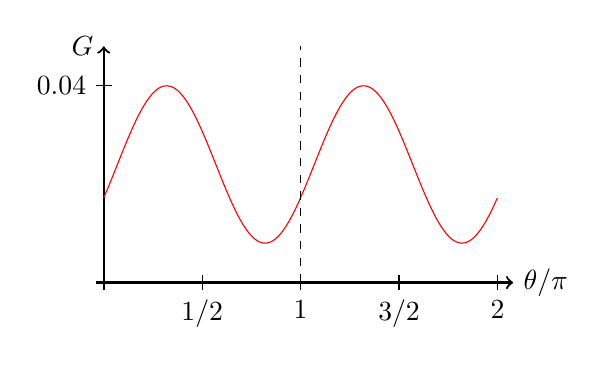
\begin{tikzpicture}
				\draw[thick,->] (-0.1, 0) -- (5.2, 0) node[right] {$\theta/\pi$};
				\draw[thick,->] (0,-0.1) -- (0, 3) node[left] {$G$};
				\draw (0.1, 2.5) -- (-0.1, 2.5) node[left] {$0.04$};
				\draw (1.25, 0.1) -- (1.25, -0.1) node[below] {$1/2$};
				\draw (2.5, 0.1) -- (2.5, -0.1) node[below] {$1$};
				\draw (3.75, 0.1) -- (3.75, -0.1) node[below] {$3/2$};
				\draw (5, 0.1) -- (5, -0.1) node[below] {$2$};
				\draw[red, smooth] plot[domain=0:5,samples=100]
				({\x},{sin(4*pi/5*deg(\x)-25)+1.5});
				\draw[dashed] (2.5, 0) -- (2.5, 3);
			\end{tikzpicture}
		\end{center}
	\item Initial energy $E_0 = 0.9$. We now find asymmetry in $\theta$ and a
		peak near $\theta = \pi/2$, indicating some preference in initial
		conditions. $G$ is also slightly larger.
		\begin{center}
			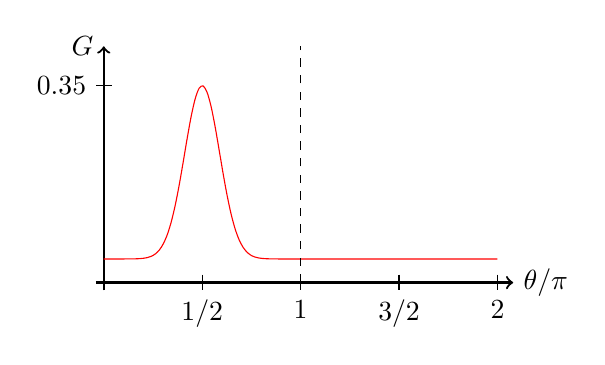
\begin{tikzpicture}
				\draw[thick,->] (-0.1, 0) -- (5.2, 0) node[right] {$\theta/\pi$};
				\draw[thick,->] (0,-0.1) -- (0, 3) node[left] {$G$};
				\draw (0.1, 2.5) -- (-0.1, 2.5) node[left] {$0.35$};
				\draw (1.25, 0.1) -- (1.25, -0.1) node[below] {$1/2$};
				\draw (2.5, 0.1) -- (2.5, -0.1) node[below] {$1$};
				\draw (3.75, 0.1) -- (3.75, -0.1) node[below] {$3/2$};
				\draw (5, 0.1) -- (5, -0.1) node[below] {$2$};
				\draw[red,smooth] plot[domain=0:5,samples=100]
				({\x},{0.3+2.2*exp(-(\x-1.25)*(\x-1.25)*10)});
				\draw[dashed] (2.5, 0) -- (2.5, 3);
			\end{tikzpicture}
		\end{center}
	\item Initial energy $E_0 = 1.0001$. A `minimal seed' is clearly
		identified for transition, i.e. the first time an initial condition
		exists which will move to another basin of attraction. Note that $G$
		is significantly larger despite a small increase in $E_0$: this is
		indicate of the fact the trajectory moves far from the origin,
		approaching the $T$ fixed point and consequently the energy (distance
		from origin) is much larger.
		\begin{center}
			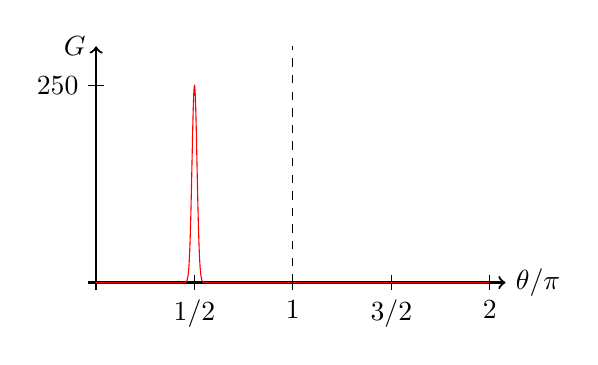
\begin{tikzpicture}
				\draw[thick,->] (-0.1, 0) -- (5.2, 0) node[right] {$\theta/\pi$};
				\draw[thick,->] (0,-0.1) -- (0, 3) node[left] {$G$};
				\draw (0.1, 2.5) -- (-0.1, 2.5) node[left] {$250$};
				\draw (1.25, 0.1) -- (1.25, -0.1) node[below] {$1/2$};
				\draw (2.5, 0.1) -- (2.5, -0.1) node[below] {$1$};
				\draw (3.75, 0.1) -- (3.75, -0.1) node[below] {$3/2$};
				\draw (5, 0.1) -- (5, -0.1) node[below] {$2$};
				\draw[red,smooth] plot[domain=0:5,samples=500]
				({\x},{2.5*exp(-(\x-1.25)*(\x-1.25)*500)});
				\draw[dashed] (2.5, 0) -- (2.5, 3);
			\end{tikzpicture}
		\end{center}
\end{itemize}

\end{document}
